%%%%%%%%%%%%%%%%%%%%%%%%%%%%%%%%%%%%%%%%%
% University Assignment Title Page 
% LaTeX Template
% Version 1.0 (27/12/12)
%
% This template has been downloaded from:
% http://www.LaTeXTemplates.com
%
% Original author:
% WikiBooks (http://en.wikibooks.org/wiki/LaTeX/Title_Creation)
%
% License:
% CC BY-NC-SA 3.0 (http://creativecommons.org/licenses/by-nc-sa/3.0/)
% 
% Instructions for using this template:x
% This title page is capable of being compiled as is. This is not useful for 
% including it in another document. To do this, you have two options: 
%
% 1) Copy/paste everything between \begin{document} and \end{document} 
% starting at \begin{titlepage} and paste this into another LaTeX file where you 
% want your title page.
% OR
% 2) Remove everything outside the \begin{titlepage} and \end{titlepage} and 
% move this file to the same directory as the LaTeX file you wish to add it to. 
% Then add \input{./title_page_1.tex} to your LaTeX file where you want your
% title page.
%
%%%%%%%%%%%%%%%%%%%%%%%%%%%%%%%%%%%%%%%%%
%\title{Title page with logo}
%----------------------------------------------------------------------------------------
%   PACKAGES AND OTHER DOCUMENT CONFIGURATIONS
%----------------------------------------------------------------------------------------

\documentclass[10pt]{article}
\usepackage{graphicx}
\usepackage[colorinlistoftodos]{todonotes}

\usepackage[utf8]{inputenc}
% Use times if you have the font installed; otherwise, comment out the
% following line.
%\usepackage[latin]{inputenc}
\usepackage[english]{babel}
\usepackage[T1]{fontenc}
\usepackage{tgtermes}
\usepackage{float, caption}
\usepackage{subcaption}
\usepackage[export]{adjustbox}

\usepackage{amsfonts}
\usepackage{amsmath}
%\usepackage{bbold}
%\usepackage{multirow}
\usepackage{amsthm,amssymb}
\renewcommand{\qedsymbol}{$\blacksquare$}
\newcommand\independent{\protect\mathpalette{\protect\independenT}{\perp}}
\def\independenT#1#2{\mathrel{\rlap{$#1#2$}\mkern2mu{#1#2}}}
\usepackage{graphicx} % Required for including images
\graphicspath{{figures/}} % Directory in which figures are stored

\usepackage{xspace}
\usepackage{multirow}
\usepackage{array}
\usepackage{graphicx}
\usepackage{latexsym}
\usepackage{mathtools}
\usepackage{listings}
\usepackage{times}
\usepackage{indentfirst}
\usepackage{algorithm}% http://ctan.org/pkg/algorithms
\usepackage[noend]{algpseudocode}% http://ctan.org/pkg/algorithmicx
\renewcommand{\algorithmicrequire}{\textbf{Input  :}}  
\renewcommand{\algorithmicensure}{\textbf{Output:}}
\renewcommand{\baselinestretch}{1.6}

% The preamble here sets up a lot of new/revised commands and
% environments.  It's annoying, but please do *not* try to strip these
% out into a separate .sty file (which could lead to the loss of some
% information when we convert the file to other formats).  Instead, keep
% them in the preamble of your main LaTeX source file.


% The following parameters seem to provide a reasonable page setup.

\topmargin 0.0cm
\oddsidemargin 0.15cm
\textwidth 16cm 
\textheight 22cm
\footskip 1.0cm
\setlength{\parindent}{2em}


%The next command sets up an environment for the abstract to your paper.

\newenvironment{sciabstract}{%
	\begin{quote} \bf}
	{\end{quote}}


% If your reference list includes text notes as well as references,
% include the following line; otherwise, comment it out.

\renewcommand\refname{References and Notes}

% The following lines set up an environment for the last note in the
% reference list, which commonly includes acknowledgments of funding,
% help, etc.  It's intended for users of BibTeX or the {thebibliography}
% environment.  Users who are hand-coding their references at the end
% using a list environment such as {enumerate} can simply add another
% item at the end, and it will be numbered automatically.

\newcounter{lastnote}
\newenvironment{scilastnote}{%
\setcounter{lastnote}{\value{enumiv}}%
\addtocounter{lastnote}{+1}%
\begin{list}%
{\arabic{lastnote}.}
{\setlength{\leftmargin}{.15in}}
{\setlength{\labelsep}{.5em}}}
{\end{list}}

\begin{document}

\begin{titlepage}

\newcommand{\HRule}{\rule{\linewidth}{0.5mm}} % Defines a new command for the horizontal lines, change thickness here

\center % Center everything on the page
 
%----------------------------------------------------------------------------------------
%   HEADING SECTIONS
%----------------------------------------------------------------------------------------

\textsc{\LARGE Ecole Nationale des Ponts et Chaussées}\\[1.5cm] % Name of your university/college
\textsc{\Large Optimisation et Contrôle}\\[0.5cm] % Major heading such as course name


%----------------------------------------------------------------------------------------
%   TITLE SECTION
%----------------------------------------------------------------------------------------

\HRule \\[0.4cm]
{ \huge \bfseries Projet sur les reseaux de distribution d'eau}\\[0.4cm] % Title of your document
\HRule \\[1.5cm]
 
%----------------------------------------------------------------------------------------
%   AUTHOR SECTION
%----------------------------------------------------------------------------------------

\begin{center}

Author: \emph{\\ \vspace{0.8em} Matthieu TOULEMENT \\ Tong ZHAO}

\end{center}


% If you don't want a supervisor, uncomment the two lines below and remove the section above
%\Large \emph{Author:}\\
%John \textsc{Smith}\\[3cm] % Your name

%----------------------------------------------------------------------------------------
%   DATE SECTION
%----------------------------------------------------------------------------------------

{\large Mai 2017}\\[2cm] % Date, change the \today to a set date if you want to be precise

%----------------------------------------------------------------------------------------
%   LOGO SECTION
%----------------------------------------------------------------------------------------


\includegraphics[width=10em]{header_logo.png}\\[1cm] % Include a department/university logo - this will require the graphicx package
 
%----------------------------------------------------------------------------------------

\vfill % Fill the rest of the page with whitespace

\end{titlepage}

\section{Présentation du problème}

On se concentre sur le problème de la résolution des équations décrivant l'état d'équilibre d'un réseau de distribution d'eau potable au cours de ce projet.

\begin{center}
  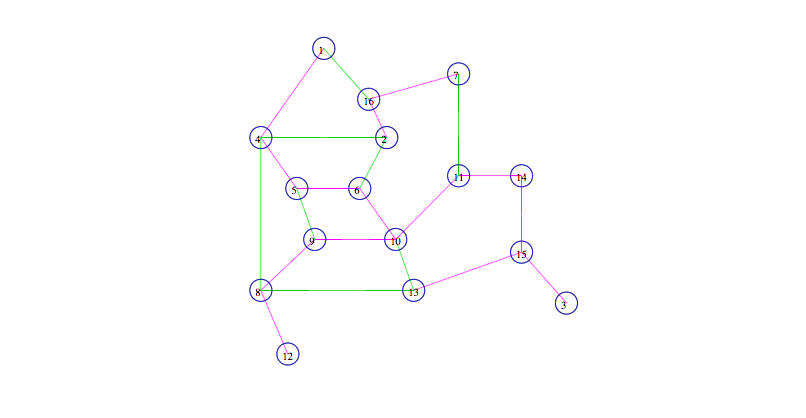
\includegraphics[width=20em]{reseau.png}
  \captionof{figure}{Un réseau d'eau potable}
\end{center}

\subsection{Modélisation du problème}

Le réseau est modélisé par un graphe orienté. L'ensemble des sommets $\mathcal{N}$ est de cardinalit $m$ tandis que l'ensemble des arcs $\mathcal{A}$ de cardinalité n. Parmi les sommets se trouvent des réservoirs $\mathcal{N}_r$ et des puits de demande $\mathcal{N}_d$ de cardinalités respectives $m_r$ et $m_d$.

On impose la connexité du graphe qui se traduit par $n \geqslant m-1$. On définit la matrice d'incidence $A$, son rang vaut $m-1$

On définit de plus les entités suivantes : 
\begin{itemize}
\item f : vecteur des flux aux noeuds
\item p : vecteur des pressions aux noeuds
\item r : vecteur des résistances des arcs
\item q : vecteur des débits dans les arcs
\end{itemize}

\subsection{Equations du modèle}
Les équations décrivant les états d'équilibres sont : 
\begin{itemize}
\item La première loi de Kirchoff : $Aqf- f= 0 $
\item La seconde loi de Kirchoff  et loi d'Ohm non linéaire: $A^Tp + r\bullet q \bullet \vert q\vert =0$
\end{itemize}


\subsection{Problème d'optimisation}

L'énergie du réseau s'écrit : 
\begin{equation}
\overline{J}(q, f_r) = \frac{1}{3}\sum_{\alpha \in \mathcal{A}} r_\alpha q_\alpha^2 \vert q_\alpha \vert + \sum_{i\in \mathcal{N}_r} p_i f_i
\end{equation}
Trouver l'équilibre revient alors à résoudre le problème : 
\begin{equation}
\underset{Aq-f = 0}{\underset{q\in \mathbb{R}^{n}}{min}< q, r\bullet q\bullet \vert q\vert> + <p, f_r>}
\end{equation}
La partition du graphe en réservoirs et puits de demande induit une partition de la matrice $A$ et des vecteurs $p$ et $f$. 
Donc  la contrainte est équivalente à :
\begin{equation}
A_rq = f_r 
\end{equation}
et
\begin{equation}
A_dq = f_d 
\end{equation}

Nous pouvons donc réécrire le problème comme : 
\begin{equation}
\underset{A_dq-f_d = 0}{\underset{q\in \mathbb{R}^{n}}{min}< q, r\bullet q\bullet \vert q\vert> + <p, A_rq>}
\end{equation}


Comme la matrice $A_d$ est de rang plein, on peut en extraire une matrice carré de taille $m_d$ inversible $A_{d,T}$. En posant  $A_d = (A_{d,T} A_{d,c})$, $q = (q_T q_c)^T$ la contrainte du problème (5) se réécrit : 
\begin{equation}
A_{d,T}q_T + A_{d,c}q_c = f_d
\end{equation}
puis 
\begin{equation}
q_T = A_{d,T}^{-1}(f_d - A_{d,c}q_c)
\end{equation}

On peut donc réécrire le problème d'optimisation sous la forme : 


\begin{equation}
\underset{q_c \in \mathcal{R}^{n - m_d}}{min} \frac{1}{3}<q^{(0)} + B*q_c, r \bullet(q^{(0)} + B*q_c)\bullet \vert q^{(0)} + B*q_c\vert > + <p_r, A_r(q^{(0)} + B*q_c)>
\end{equation}

$$\mbox{où: } q^{(0)} = A_{d,T}^{-1}f_d \mbox{ et } B = (\begin{array}{c} - A_{d,T}^{-1}A_{d,c} \\ I_{n-m_d} \end{array})$$


\section{Première séance de TP}

Dans cette partie, on s'intéresse au problème primal d'optimisation sans contrainte.

\vspace{-1.5em}
\begin{align}
  min_{q_C \in \mathbb{R}^{n-m_d}} \frac{1}{3} \left \langle q^{(0)} + B q_c, r \bullet (q^{(0)} + B q_c) \bullet |q^{(0)} + B q_c| \right \rangle + \left \langle p_r, A_r(q^{(0)} + B q_c) \right \rangle
\end{align}

\subsection{Calcul du gradient}

D'abord, on calcule le gradient du premier terme.

\vspace{-1.5em}
\begin{align}
  f_1 (q_c) = \left \langle q^{(0)} + B q_c, r \bullet (q^{(0)} + B q_c) \bullet |q^{(0)} + B q_c| \right \rangle
\end{align}

On pose $q = q^{(0)} + B q_c$ et on calcule

\vspace{-1.5em}
\begin{align}
  \cfrac{\partial f_1}{\partial q} &= \cfrac{\partial  \left \langle q, r \bullet q \bullet |q| \right \rangle}{\partial q} = \cfrac{\partial(r \bullet q \bullet q \bullet |q|)}{\partial q} = 3sign(q) \bullet r \bullet q \bullet q = 3r \bullet q \bullet |q|
\end{align}

Ensuite, on calcule le gradient du second terme.

\vspace{-1.5em}
\begin{align}
  f_2 (q_c) = \left \langle p_r, A_r (q^{(0)} + B q_c) \right \rangle
\end{align}

\vspace{-1.5em}
\begin{align}
  \cfrac{\partial f_2}{\partial q} = \cfrac{\partial (p_r \bullet A_r q)}{\partial q} = A_r^T p_r
\end{align}

Sachant que $\cfrac{\partial q}{\partial q_c} = B^T$, on calcule le gradient de la fonction $F$.

\vspace{-1.5em}
\begin{align}
  G(q_c) = \cfrac{\partial F}{\partial q_c} = \cfrac{\partial (3f_1 + f_2)}{\partial q} \cfrac{\partial q}{\partial q_c} = B^T (r \bullet q \bullet |q| + A_r^T p_r)
\end{align}

\subsection{Calcul du hessien}

On veut calculer:

\vspace{-1.5em}
\begin{align}
  H(q_c) = \cfrac{\partial G}{\partial q_c} = \cfrac{\partial (B^T(r \bullet q \bullet |q| + A_r^T p_r))}{\partial q_c}
\end{align}

On pose $d = r \bullet q \bullet |q|$, alors

\vspace{-1.5em}
\begin{align}
 H(q_c) = \cfrac{\partial (B^T d)}{\partial d} \cfrac{\partial d}{\partial q} \cfrac{\partial q}{\partial q_c} 
\end{align}

Sachant que:

\vspace{-1.5em}
\begin{align*}
  \frac{\partial d}{\partial q} &=
  \begin{bmatrix}
    \frac{\partial d_1}{\partial q_1} & \bullet & \frac{\partial d_1}{\partial q_n} \\
    \vdots & \ddots & \vdots \\
    \frac{\partial d_n}{\partial q_1} & \bullet & \frac{\partial d_n}{\partial q_n}
  \end{bmatrix} \mbox{\ \ \ d'où \ \ } \frac{\partial d_i}{\partial q_j} =
  \begin{cases} 
    2r_i|q_i|,  & i = j \\
    0, & i \ne j
  \end{cases}
\end{align*}

On a:

\vspace{-1.5em}
\begin{align}
  \frac{\partial d}{\partial q} = diag((2r_i|q_i|)_{i=1 \cdots n})
\end{align}

On en déduit que:

\vspace{-1.5em}
\begin{align}
 H(q_c) = 2B^T diag((2r_i|q_i|)_{i=1 \cdots n}) B 
\end{align}

\subsection{Tester l'oracle avec deux méthodes fournies}

On teste notre oracle en l'interfaçant avec un algorithme de gradient à pas fixe et on le compare avec la fonction optim de Scilab. Les résultats sont comme suit:

\vspace{1em}

\begin{minipage}[t]{.5\textwidth}
    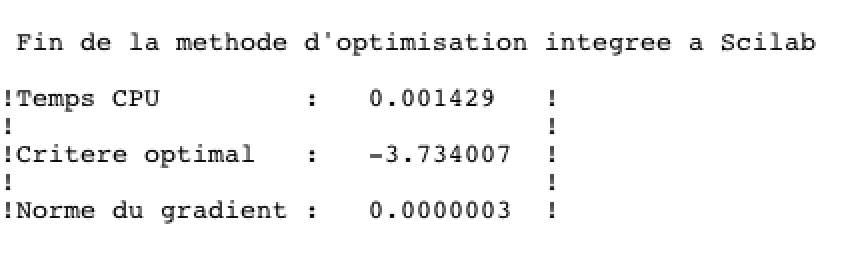
\includegraphics[width=20em]{pg_scilab.png}
\end{minipage}
\begin{minipage}[t]{.5\textwidth}
    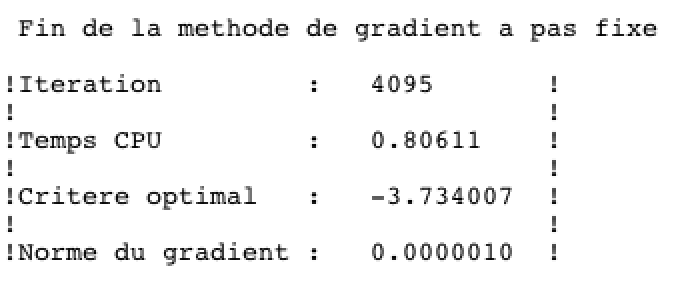
\includegraphics[width=15em]{pg_fix.png}
\end{minipage}

\begin{minipage}[t]{.5\textwidth}
  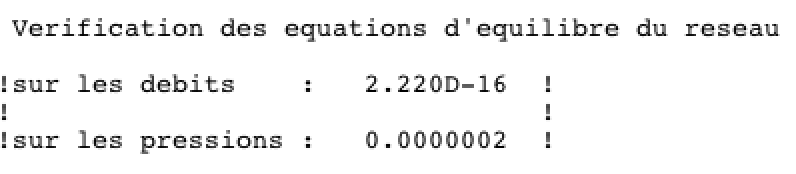
\includegraphics[width=20em]{pg_scilab_v.png}
  \captionof{figure}{\small Le calcul avec Optim\_scilab}
\end{minipage}
\begin{minipage}[t]{.5\textwidth}
  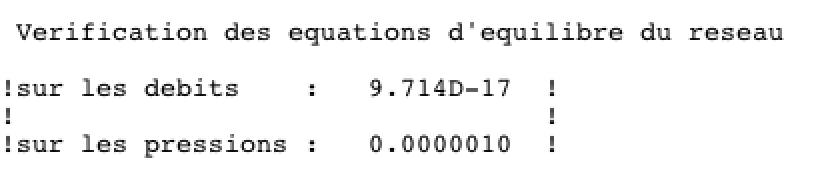
\includegraphics[width=20em]{pg_fix_v.png}
  \captionof{figure}{\small Le calcul avec Gradient\_F}
\end{minipage}

\vspace{2em}
On visualise l'évaluation de la norme du gradient (echelle logarithmique) en fonction d'itération.

\begin{center}
  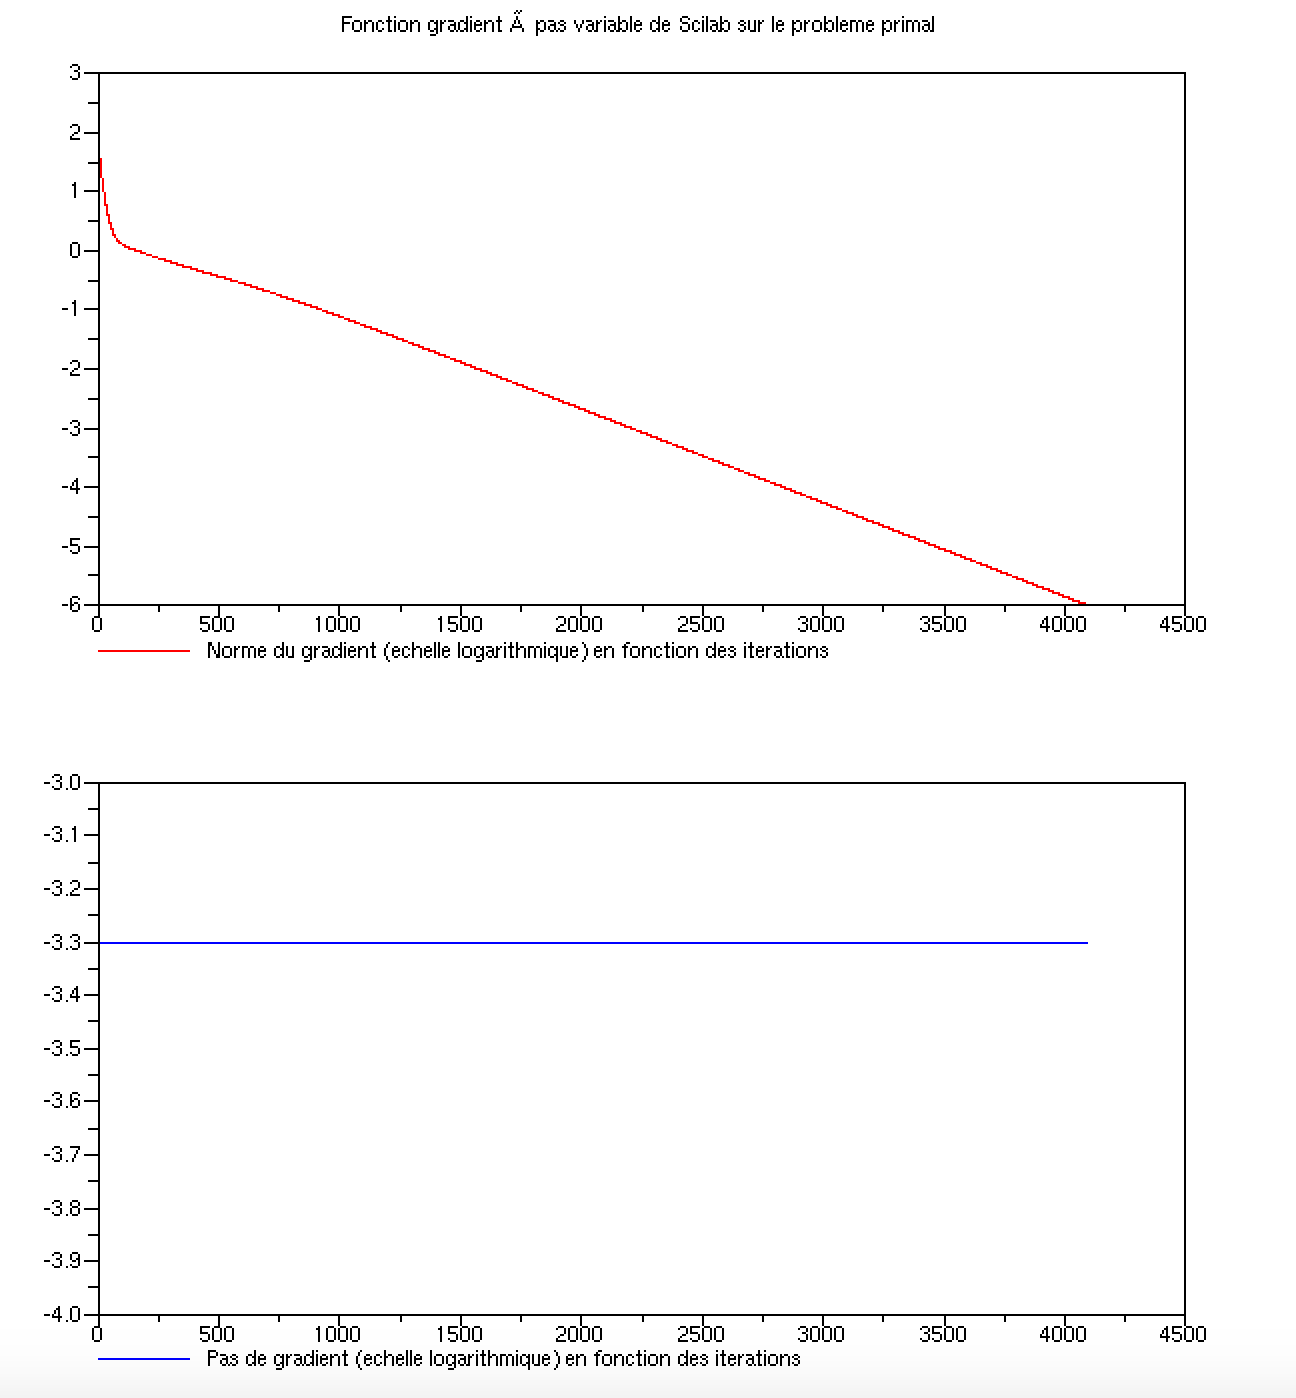
\includegraphics[width=20em]{pg_fix_f.png}
  \captionof{figure}{\small La performance du Gradient\_F}
\end{center}

A l'observation, on voit que la vitesse de convergence est assez lent donc il prend plus de temps ($\times$ 800) que la fonction optim de Scilab. De plus, la perfoemance de convergence est pire que celle de la fonction optim de Scilab.

\section{Seconde et troisième séance de TP}


Lors de cette séance nous souhaitons étudier le problème (1) à l'aide de 4 algorithmes d'optimisations différents.

\subsection{Fletcher - Lemaréchal}
 
Dans cette partie, on va programmer une recherche linéaire vérifiant les conditions de Wolfe et coder l’algorithme de gradient à pas variable utilisant cette recherche linéaire.

En prenant les notations dans l'énoncé de TP, les conditions de Wolfe sont comme suit:

\begin{itemize}
\item La fonction $f$ doit décroître de manière significative
  $$f(x^{(k)} + \alpha^{(k)} d^{(k)}) \le f(x^{(k)}) + \omega_1 \alpha^{(k)} {g^{(k)}}^T d^{(k)}$$
\item Le pas $\alpha^{(k)}$ doit être suffisamment grand
  $$(\nabla f(x^{(k)} + \alpha^{(k)} d^{(k)}))^T d^{(k)} \ge \alpha_2 {g^{(k)}}^T d^{(k)}$$
\end{itemize}

avec $0 < \omega_1 < \omega_2 < 1$.

On utilise {\it Gradient\_W.sci} pour tester le Wolfe et on obtient le résultat suivant.

\begin{center}
  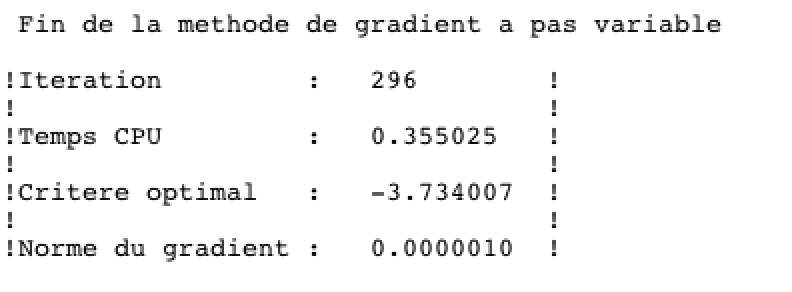
\includegraphics[width=20em]{wolfe.png}
  
  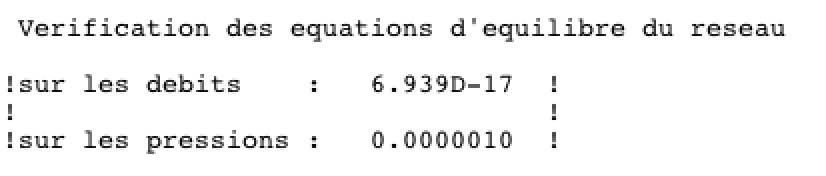
\includegraphics[width=20em]{wolfe_v.png}
  \captionof{figure}{\small La performance du Grandient\_W}

  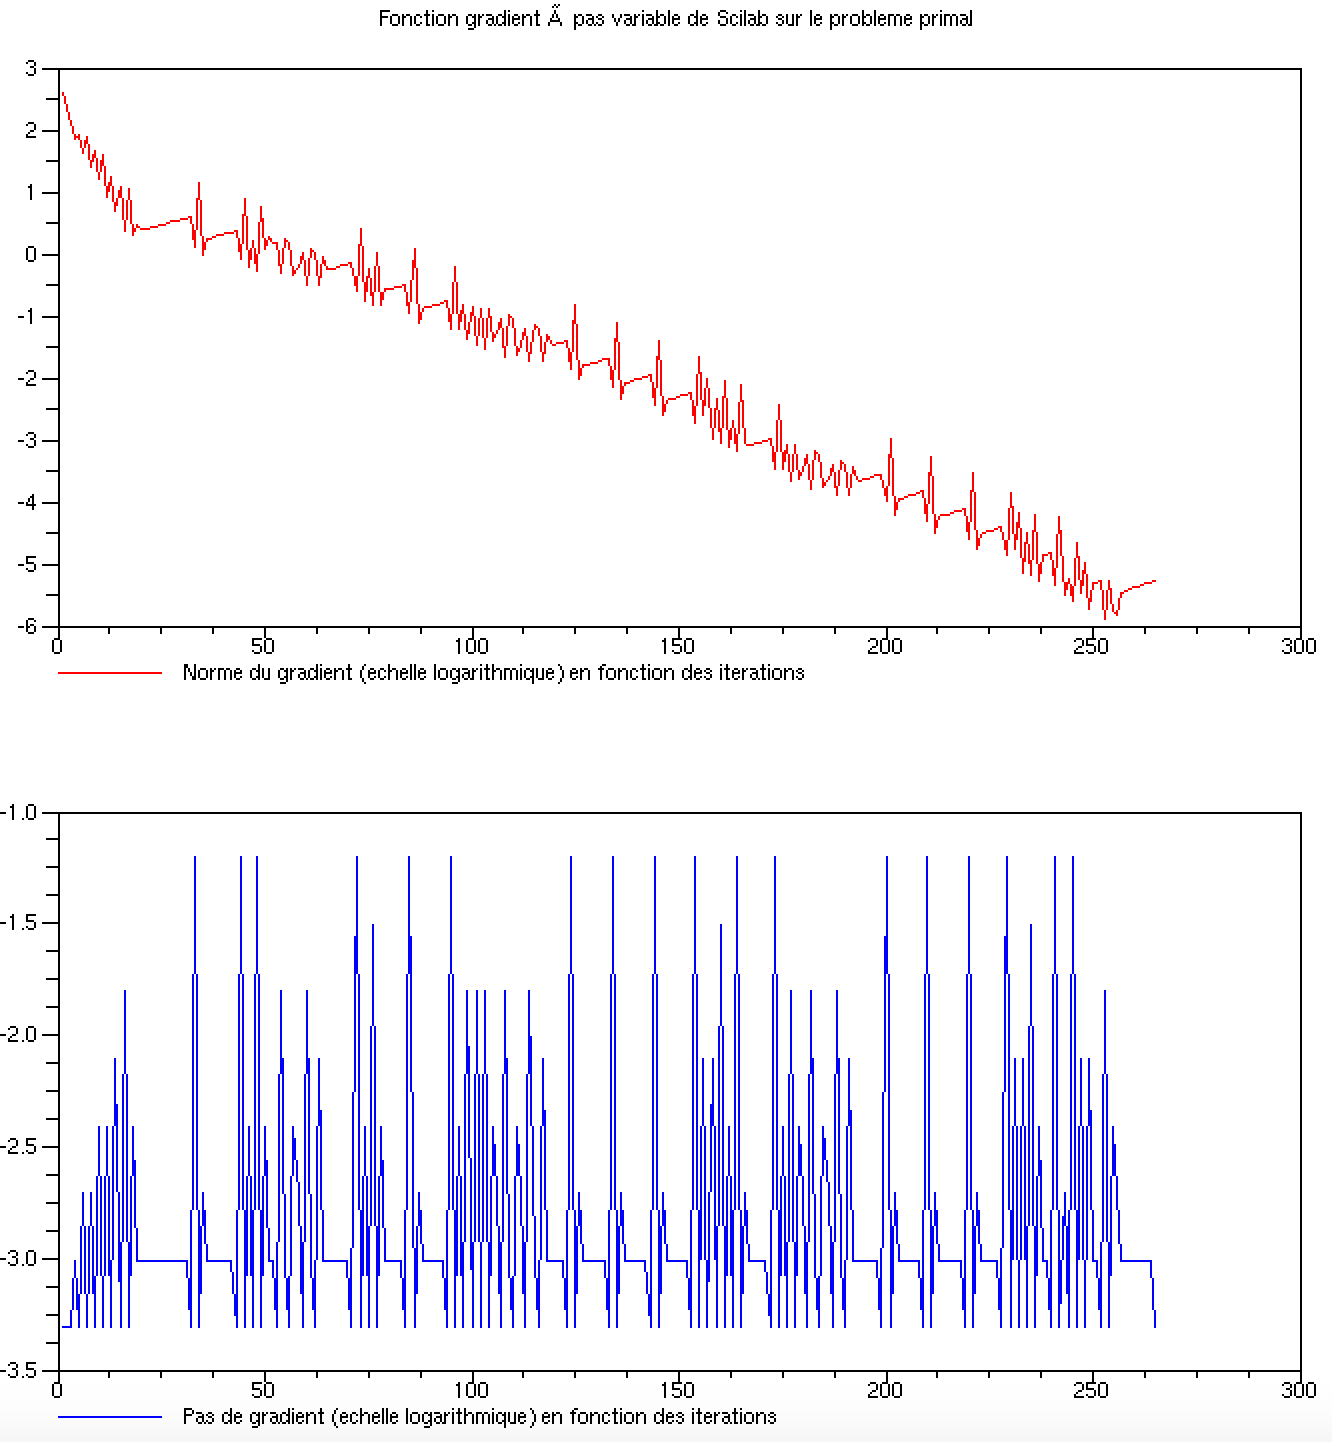
\includegraphics[width=20em]{wolfe_f.png}
  \captionof{figure}{\small La performance du Grandient\_W}
\end{center}

A l'observation, on voit que le gradient augmente de temps en temps, surtout quadn le pas change.

\subsection{Polak - Ribière}

L'algorithme de Polak-Ribière est comme suit:

\begin{algorithm}
\caption{Polak-Pibère}
\begin{algorithmic}[1]
  \State Initialiser $x_0$
  \State $f_0 = f(x_0),\ \ g_0 = f'(x_0),\ \ d_0 = -g_0$
  \State $x_1 = x_0 + d_0$
  \State $n=1$
  \While{True}
    \If{$\| g(x_n) \| \le \epsilon$}
      return
    \EndIf

    \State $\beta_n = \cfrac{g_n^T (g_n - g_{n-1})}{\| g_{n-1} \|_2^2}$
    \State $d_n = -g_n + \beta_n d_{n-1}$
    \State $\alpha_n$ calculé par Wolfe
    \State $x_{n+1} = x_n + \alpha_n * d_n$
    \State $n = n+1$
  \EndWhile
\end{algorithmic}
\end{algorithm}

Le résultat est présenté suivant:

\begin{center}
  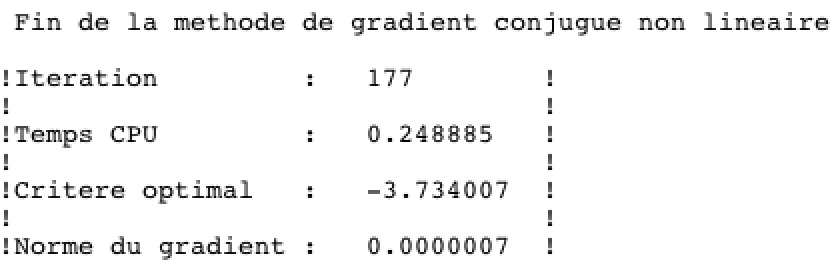
\includegraphics[width=20em]{conj.png}
  
  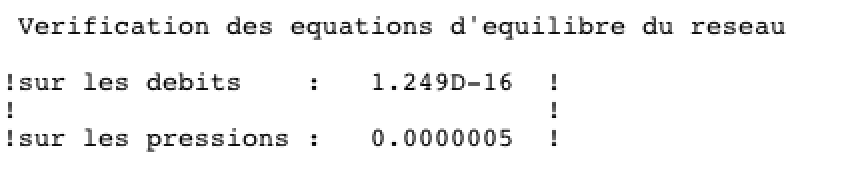
\includegraphics[width=20em]{conj_v.png}
  \captionof{figure}{\small La performance du Grandient\_Conj}

  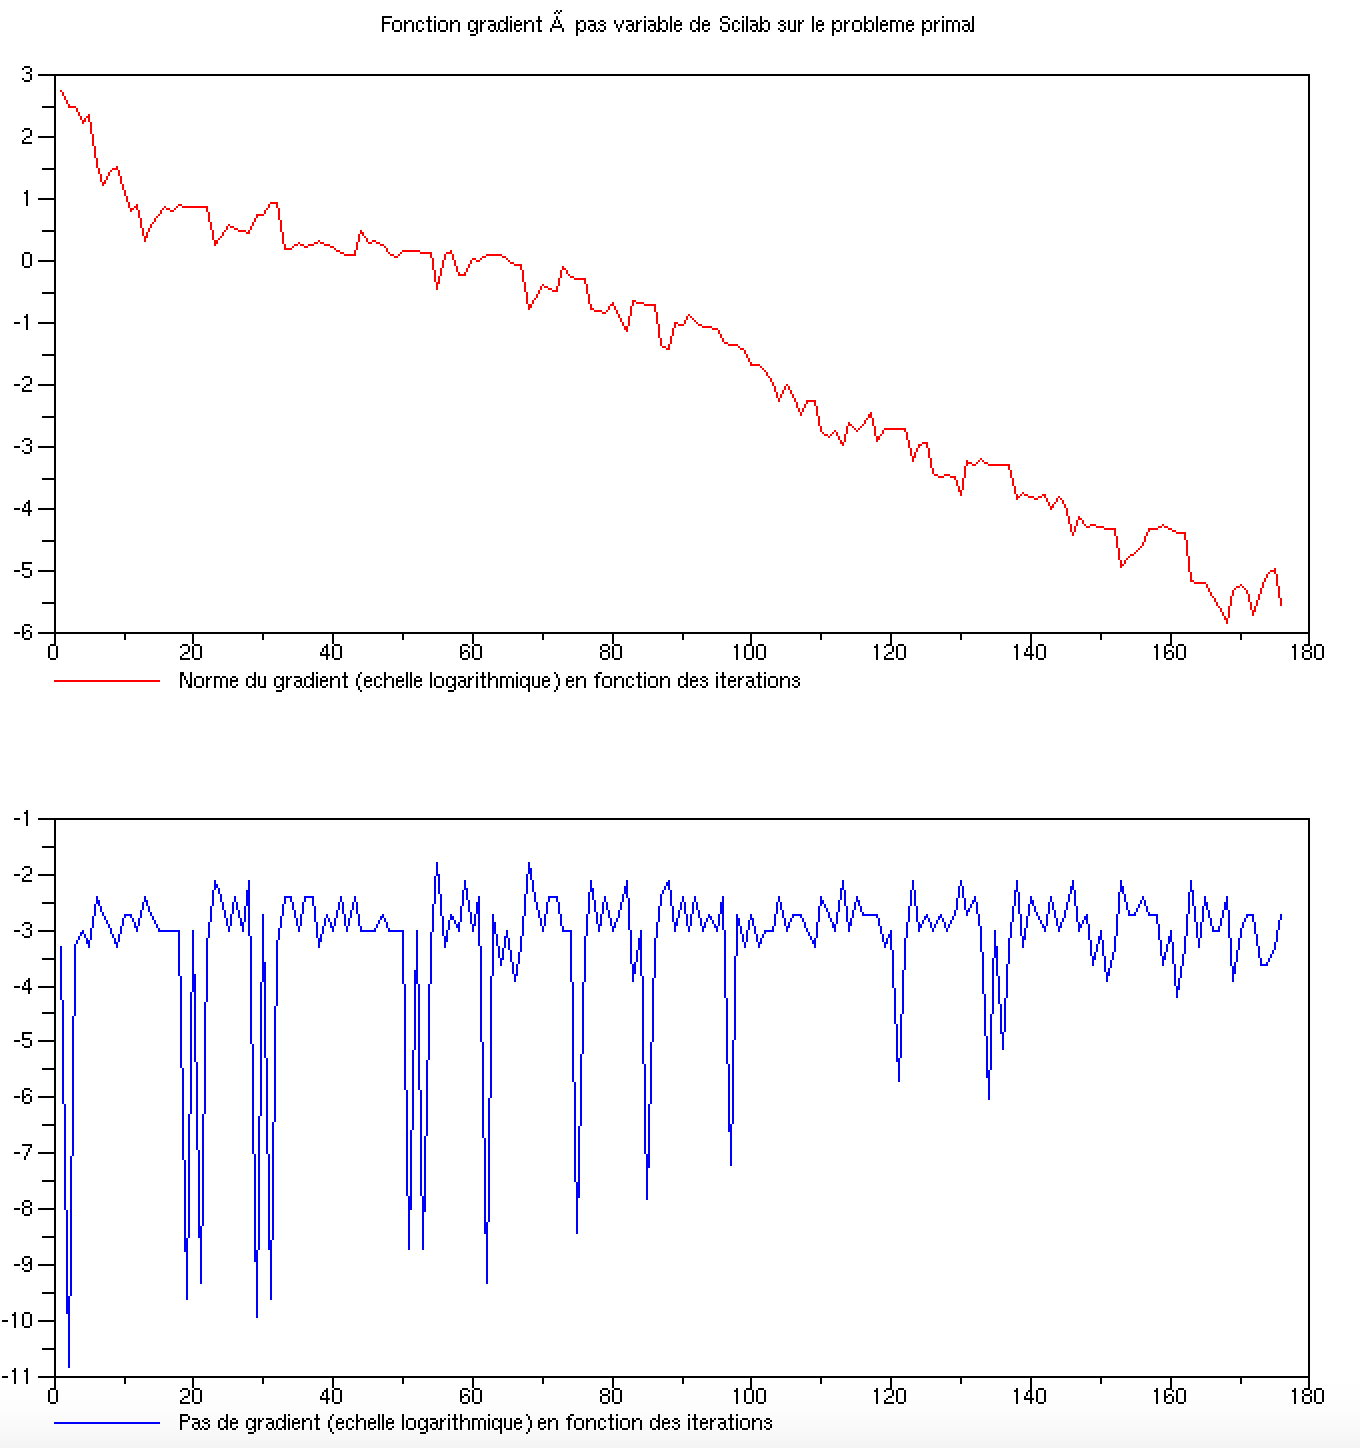
\includegraphics[width=20em]{conj_f.png}
  \captionof{figure}{\small La performance du Grandient\_Conj}
\end{center}

A l'aide de algorithme de Polak - Ribière, la vitesse augmente et le changement de pas est plus doux.

\subsection{BFGS}

L'idée principale de cette méthode est d'approximer la matrice hessienne pour éviter le calcul coûteux.

On pose $\delta_x^{(k)} = x^{(k+1)} - x^{(k)}$ et $\delta_G^{(k)} = \nabla J(x^{(k+1)}) - \nabla J(x^{(k)}$, et chaque itération on utilise la formule suivante pour mettre à jour l'approximation de la matrice de Hessienne:

$$W^{(k+1)} = (I - \cfrac{\delta_x^{(k)} {\delta_G^{(k)}}^T}{{\delta_G^{(k)}}^T} \delta_x^{(k)}) W^{(k)} (I - \cfrac{\delta_G^{(k)} {\delta_x^{(k)}}^T}{{\delta_G^{(k)}}^T} \delta_x^{(k)}) + \cfrac{\delta_x^{(k)} {\delta_x^{(k)}}^T}{{\delta_G^{(k)}}^T} \delta_x^{(k)}$$

En prenant $d_k = - W^{(k)} G^{(k)}$, on calcule $x^{(k+1)} = x^{(k)} + \alpha_k d_k$ où $\alpha_k$ est optimisé par l'algorithme de Wolfe.

\begin{center}
  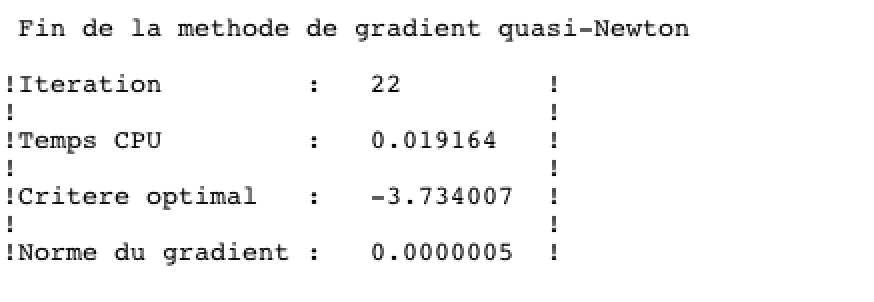
\includegraphics[width=20em]{quasi.png}
  
  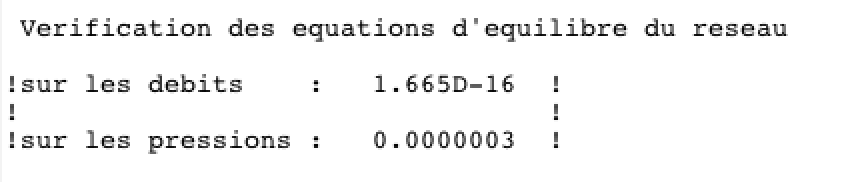
\includegraphics[width=20em]{quasi_v.png}
  \captionof{figure}{\small La performance de Quasi\_Newton}

  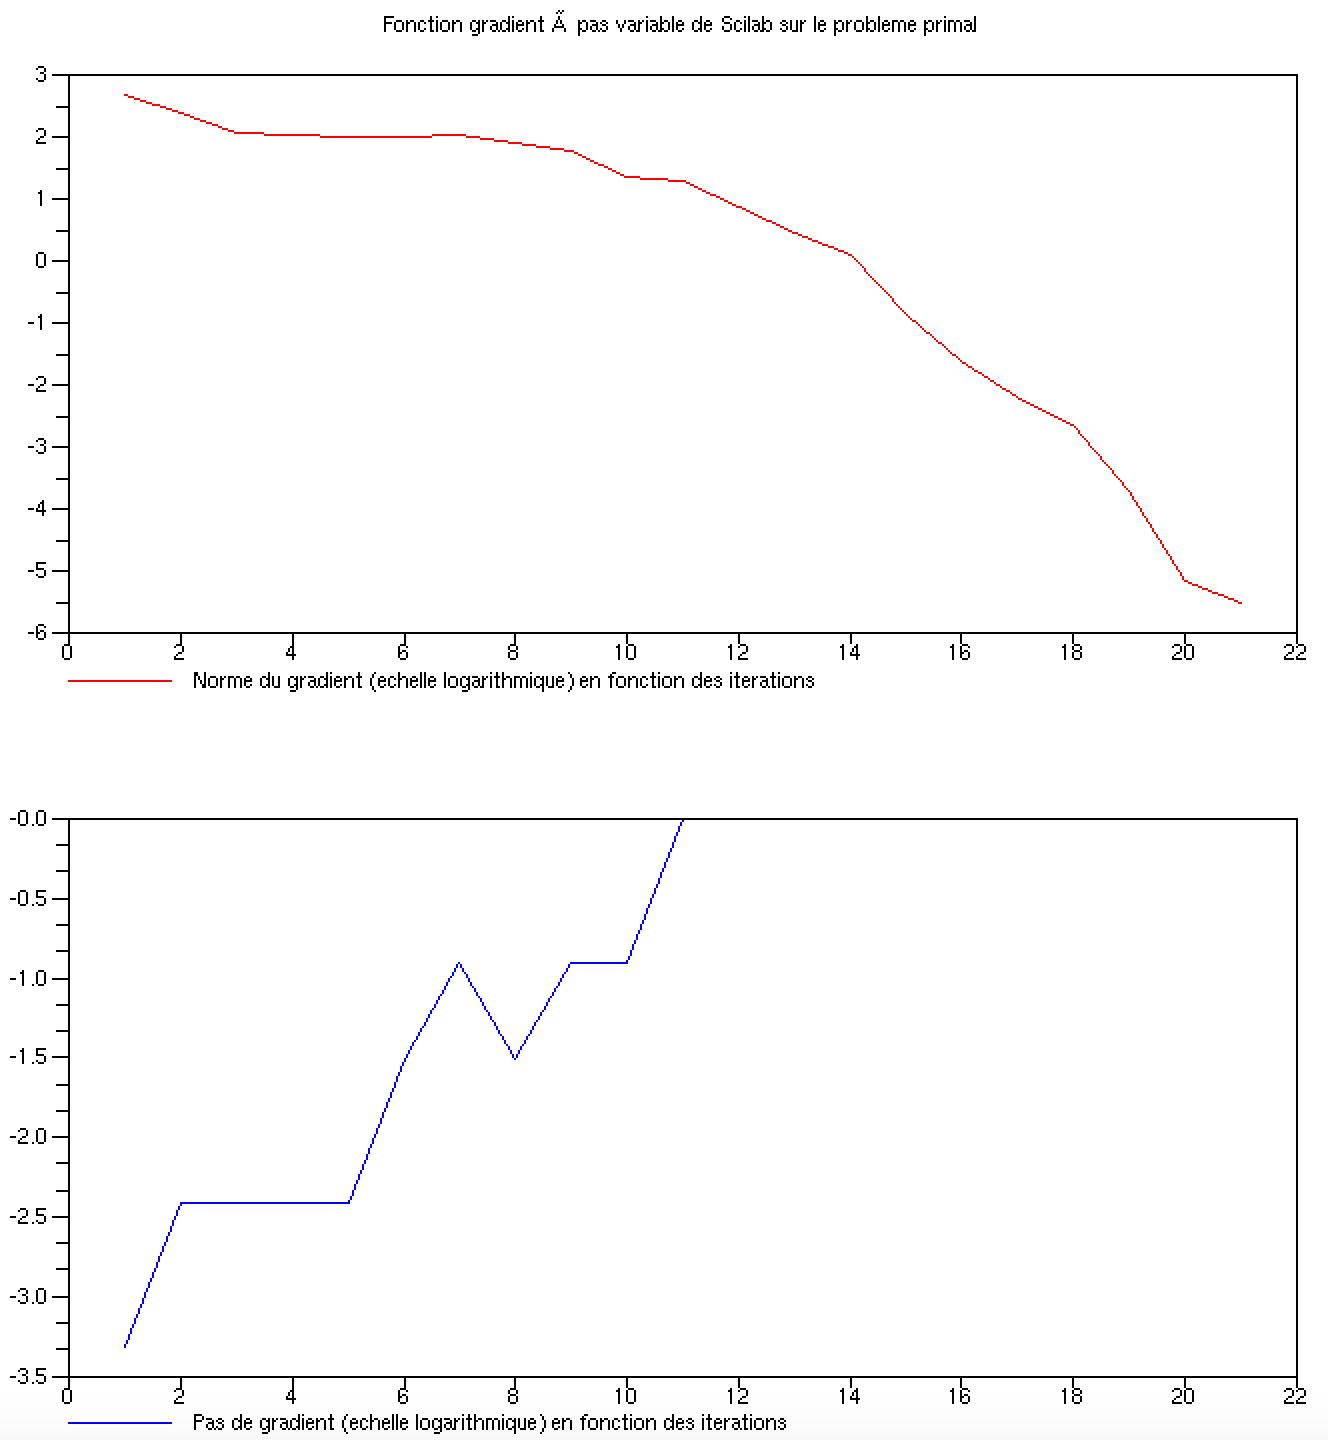
\includegraphics[width=20em]{quasi_f.png}
  \captionof{figure}{\small La performance de Quasi\_Newton}
\end{center}

A l'observation, on voit que la vitesse de convergence est assez rapide.

\subsection{Méthode de Newton}

La méthode de Netwon utilise la matrice de Hessienne pour calculer la direction de descente. On pose $d_k = - H_k^{-1} G$ et on calcule $x_{k+1} = x_k + \alpha_k d_k$.

\vspace{2em}
\begin{center}
  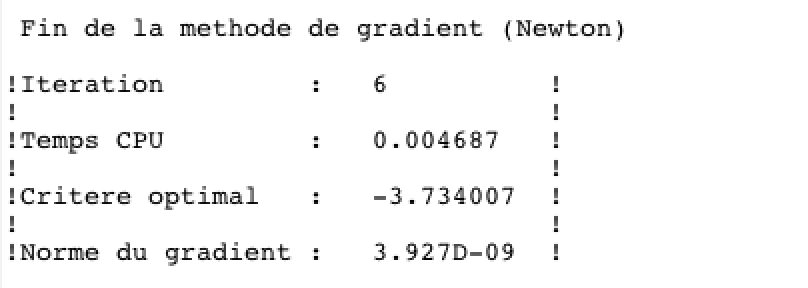
\includegraphics[width=20em]{newton.png}
  
  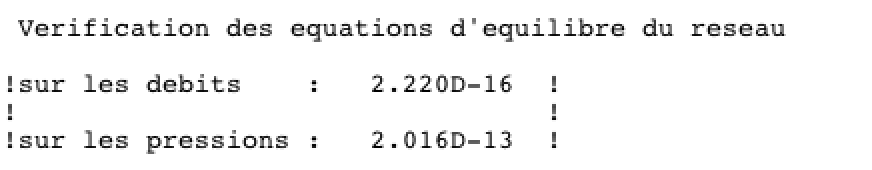
\includegraphics[width=20em]{newton_v.png}
  \captionof{figure}{\small La performance de Newton}

  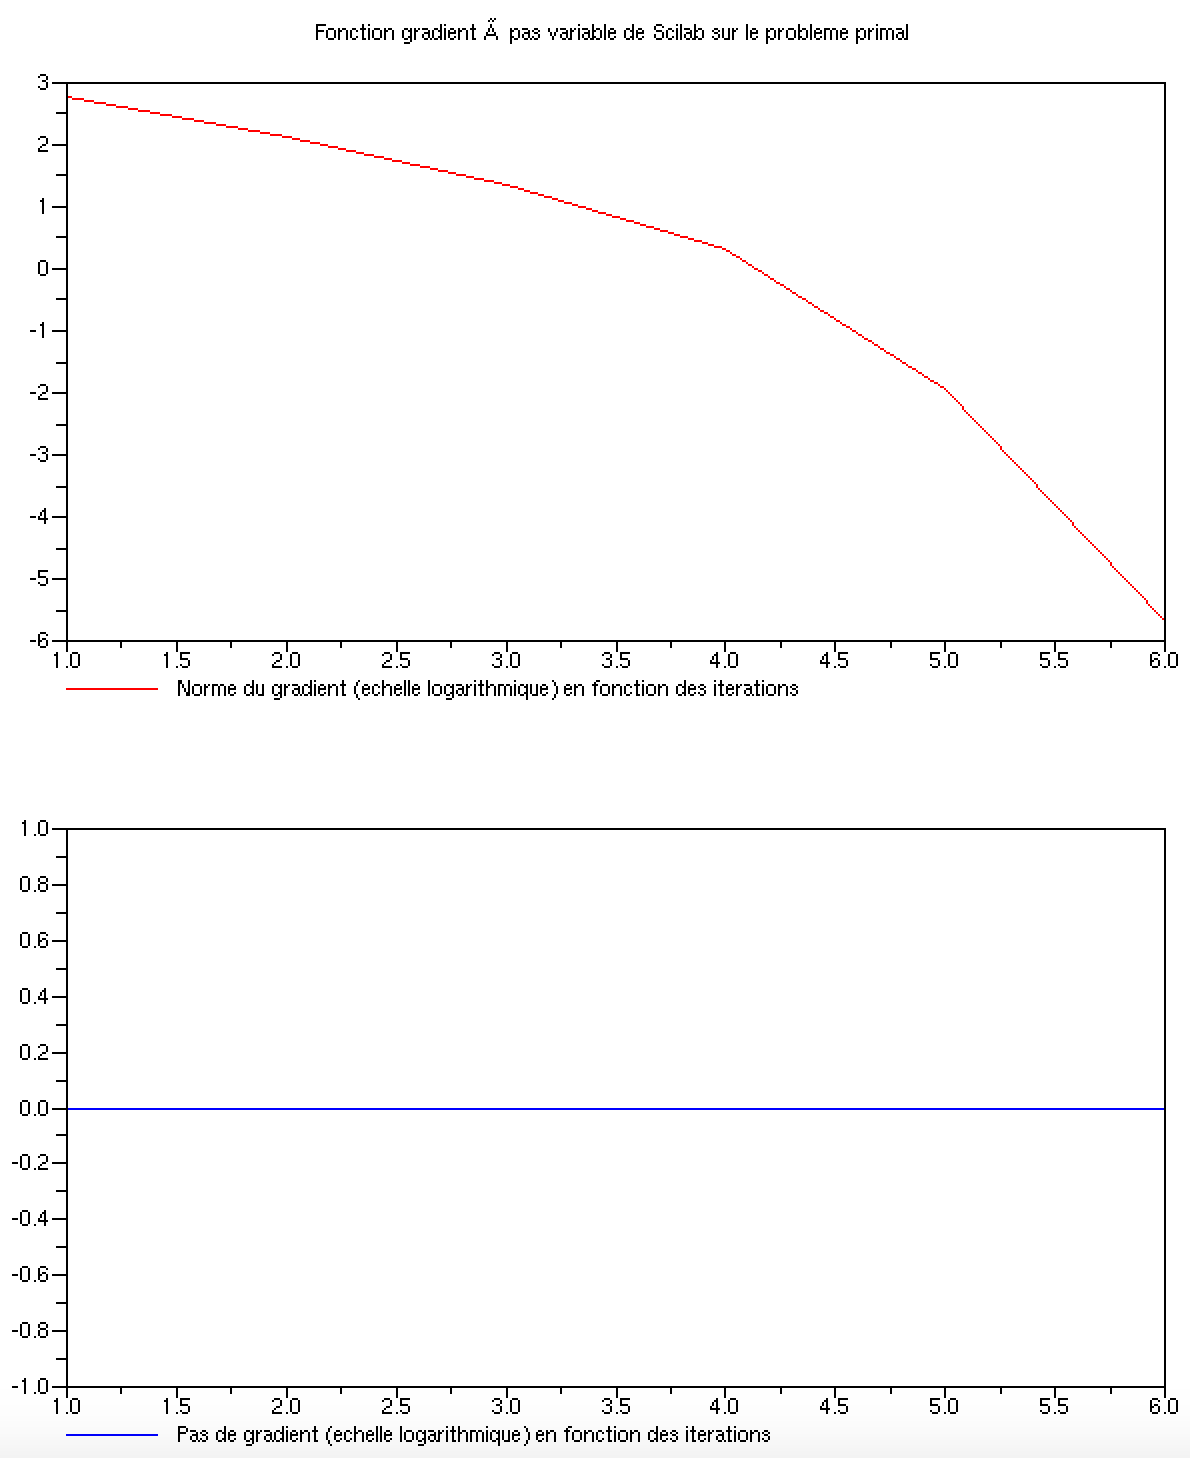
\includegraphics[width=20em]{newton_f.png}
  \captionof{figure}{\small La performance de Newton}
\end{center}


\subsection{Tableau - Comparatif des résultats}

Dans cette partie, on compare tous les algorithmes qu'on utilise et on analyse les différences entre eux.

\begin{center}
    \begin{tabular}{| l | c | c | c | c |}
    \hline
    Algorithme & Itération & Temps CPU & Critère optimal & Norme de gradient \\ \hline
    La fonction optim de Scilab & - & 0.001429 & -3.734007 & 3$\times 10^{-7}$\\ \hline  
    Le gradient à pas fixe & 4095 & 0.80611 & -3.734007 & $10^{-6}$ \\ \hline
    Le gradient à pas variable  & 296 & 0.355025 & -3.734007 & $10^{-6}$\\ \hline
    Le gradient conjugué  & 177 & 0.248885 & -3.734007 & $7\times 10^{-7}$\\ \hline
    L'algorithme de quasi-Newton & 22 & 0.019164& -3.734007 & $5\times 10^{-7}$\\ \hline
    L'algorithme de Newton & 6 & 0.004687 & -3.734007 & 3.927$\times 10^{-9}$\\ 
    \hline
    \end{tabular}
\end{center}

Au travers du tableau, on voit que l'algorithme de Newton nous donne le meilleur résultat. De plus il est le plus rapide parmi tous les algorithmes qu'on implémente par soi même. Cependant il faudrait noter que l'inverse de la matrice de Hessienne est quelque fois difficile à calculer. Dans ce cas, cet algorithme ne marche plus. On a le classement suivant:

Newton > Quasi-Newton(BFGS) > Polak-Ribière > Le gradient à pas variable > Le gradient à pas fixe

\section{Quatrième séance de TP}

Dans ce TP nous avons étudié la résolution de ce problème par la dualité. Pour primal nous considérons le problème : 

\begin{align}
  &{ \underset{q\in \mathbb{R}^n}{min} \frac{1}{3} <q, r \bullet q \bullet \vert q\vert> + <p_r, A_rq> }\\
  \nonumber &s.c. A_d q - f_d = 0
\end{align}

\paragraph{Lagrangien}

Le Lagrangien du problème s'écrit :
\begin{equation}
\mathcal{L}(q, \lambda) = \frac{1}{3} <q, r\bullet q\bullet \vert q\vert> + <p_r, A_rq> + \lambda^T(A_dq - f_d)
\end{equation}

Pour trouver les valeurs extrêmes de $\mathcal{L}$, on calcule le gradient:
\begin{equation}
  \cfrac{\partial \mathcal{L} (q, \lambda)}{\partial q} = r\bullet q \bullet |q| + A_r^T p_r + A_d^T \lambda
\end{equation}

Soit $\hat{q}$ la valeur extrême du Lagrangien, on a:

\begin{align}
  &r\bullet \hat{q} \bullet |\hat{q}| =  -( A_r^T p_r + A_d^T \lambda)\\
  &C_i = \hat{q}_i |\hat{q}_i| = - \frac{1}{r_i} (\sum_{j=1}^{m_r} A_r(j,i) p_r(j) + \sum_{j=1}^{m_d} A_d(j, i) \lambda(j)) &\forall i \in [1,n]\\
  &\hat{q}_i = -signe(C_i)\sqrt{|C_i|} &\forall i \in [1,n]\\
\end{align}

\paragraph{Fonction duale}

Le problème dual est:

\begin{equation}
  \underset{\lambda \in \mathbb{R}^{m_d}}{max} \underset{q\in \mathbb{R}^n}{min}  \mathcal{L} (q, \lambda)
\end{equation}

La fonction duale est donc de la forme : 
\begin{equation}
\forall \lambda \in \mathbb{R}^d  : H(\lambda) = \underset{q\in \mathbb{R}^n}{min} \mathcal{L} (q, \lambda) = - \frac{1}{3} \hat{q}(\lambda)^T(A_d^T\lambda + A_r^Tp_r) + p_r^TA_r\hat{q}(\lambda)
\end{equation}


\paragraph{Gradient de la fonction duale}
Ce gradient est simple à exprimer car $\hat{q}(\lambda)$ vérifie $\frac{\partial \mathcal{L}}{\partial{q}}(\hat{q}(\lambda), \lambda) = 0$


Il vient : 
\begin{equation}
\nabla H(\lambda) = \frac{ \partial \mathcal{L}}{\partial \lambda} (\hat{q}(\lambda), \lambda)
\end{equation}
Qui devient : 
\begin{equation}
\nabla H(\lambda) = A_d\hat{q}(\lambda) - f_d
\end{equation}

\paragraph{Hessien de la fonction duale}
Le hessien de la fonction duale est de la forme :
\begin{equation}
\nabla^2 H(\lambda) = A_d \nabla \hat{q}(\lambda)
\end{equation}

Pour déterminer le gradient de l'argmin : $\hat{q}(\lambda)$ procédons coordonnées par coordonnées. 
\\
$\forall i  \in [1,n], \forall j \in [1, d]$
\begin{equation}
\frac{\partial \hat{q}_i}{\partial \lambda_j} = - signe(C_i)\frac{\frac{\partial \vert C_i \vert }{\partial \lambda_j}}{2\sqrt{\vert C_i \vert}} 
\end{equation}

Comme $\frac{\partial \vert C_i \vert }{\partial \lambda_j} = \frac{1}{r_i}A_d[j,i]$ il vient : 

\begin{equation}
\frac{\partial \hat{q}_i}{\partial \lambda_j} = - signe(C_i)\frac{A_d(j,i)}{2r_i\sqrt{\vert C_i \vert}} 
\end{equation}

Ainsi en posant $\delta_i = -\frac{1}{2r_i\sqrt{\vert C_i \vert}}$ nous avons la forme simple suivante : 
\begin{equation}
\nabla \hat{q}(\lambda) = diag(\delta_1 , .. , \delta_n)A_d^T
\end{equation}

Puis, finalement nous pouvons écrire le hessien de la fonction duale : 

\begin{equation}
\nabla^2 H(\lambda) = A_ddiag(\delta_1 , .. , \delta_n)A_d^T
\end{equation}

\section{Algorithmes d'optimisation pour le problème dual}

On résoudre le problème dual à l’aide des algorithmes développés lors des séances dernières. En pratique, on s'intéresse à la minimisation de l’opposé de fonction objective $\mathcal{L}$.

D'abord on utilise la fonction optim fourni par Scilab. On affiche le résultat pour faire la comparaison avec nos algorithmes.

\begin{center}
  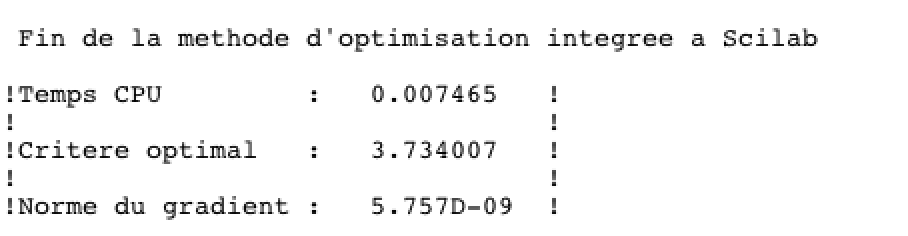
\includegraphics[width=20em,valign=t]{d_scilab.png}
  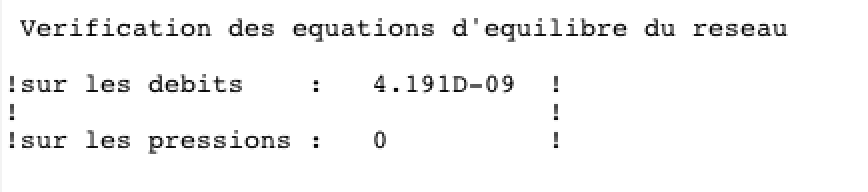
\includegraphics[width=20em,valign=t]{d_scilab_v.png}
  \captionof{figure}{\small La performance de la fonction Optim Scilab}
\end{center}

\subsection{Gradient à pas fixe}

\begin{center}
  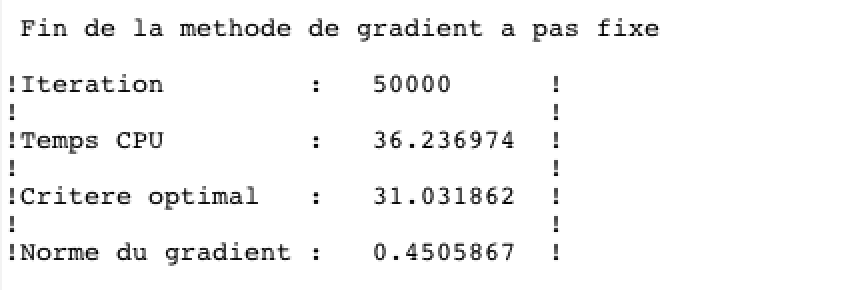
\includegraphics[width=20em,valign=t]{d_fixe.png}
  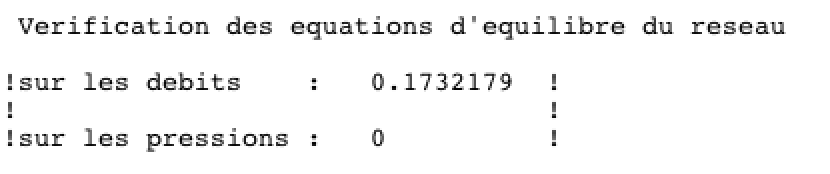
\includegraphics[width=20em,valign=t]{d_fixe_v.png}
  \captionof{figure}{\small La performance du Gradient à pas fixe}

  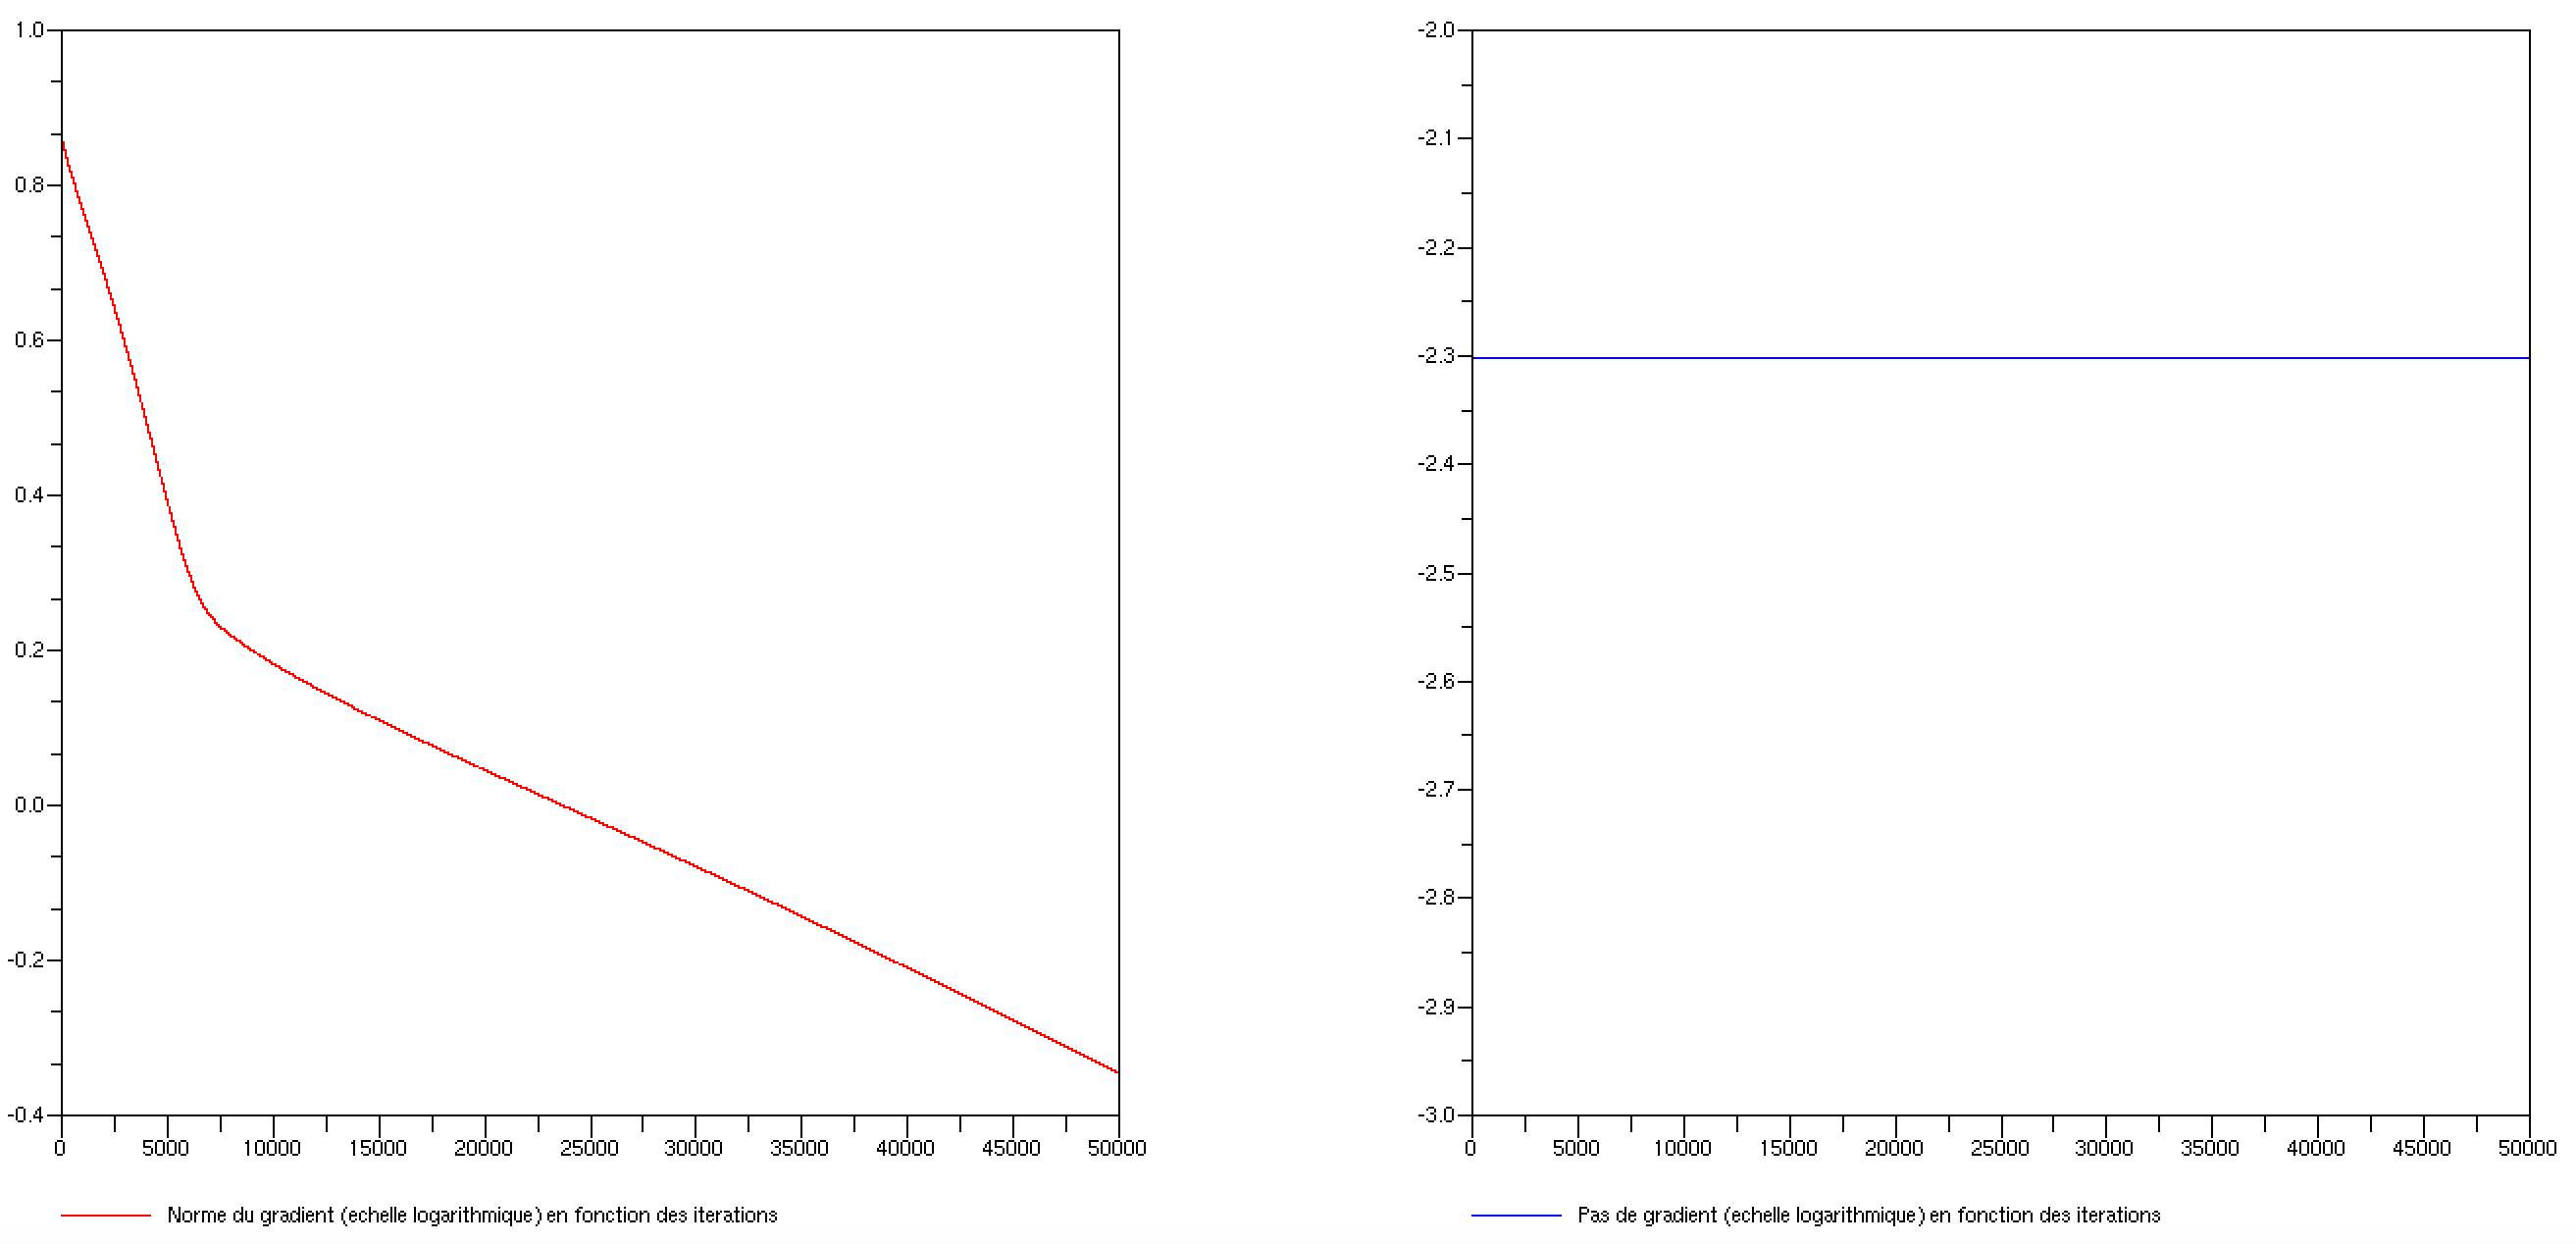
\includegraphics[width=40em,height=15em]{d_fixe_f.png}
  \captionof{figure}{\small La performance du Gradient à pas fixe}
\end{center}

A l'observation, on voit que le grqdient à pas fixe ne suffit pas à resoudre le problème dual. Bien qu'on a multiplié le nombre d'itération par 10 et le pas par 10, le résultat ne converge pas.

\subsection{Fletcher - Lemaréchal}

\begin{center}
  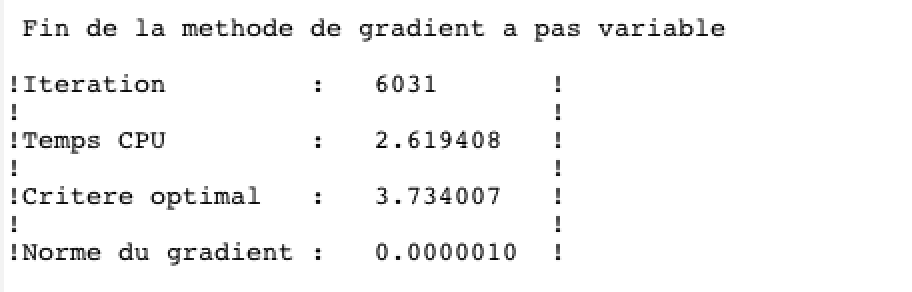
\includegraphics[width=20em,valign=t]{d_wolfe.png}
  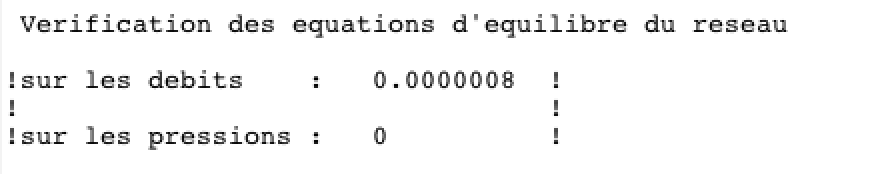
\includegraphics[width=20em,valign=t]{d_wolfe_v.png}
  \captionof{figure}{\small La performance du Gradient à pas variable}

  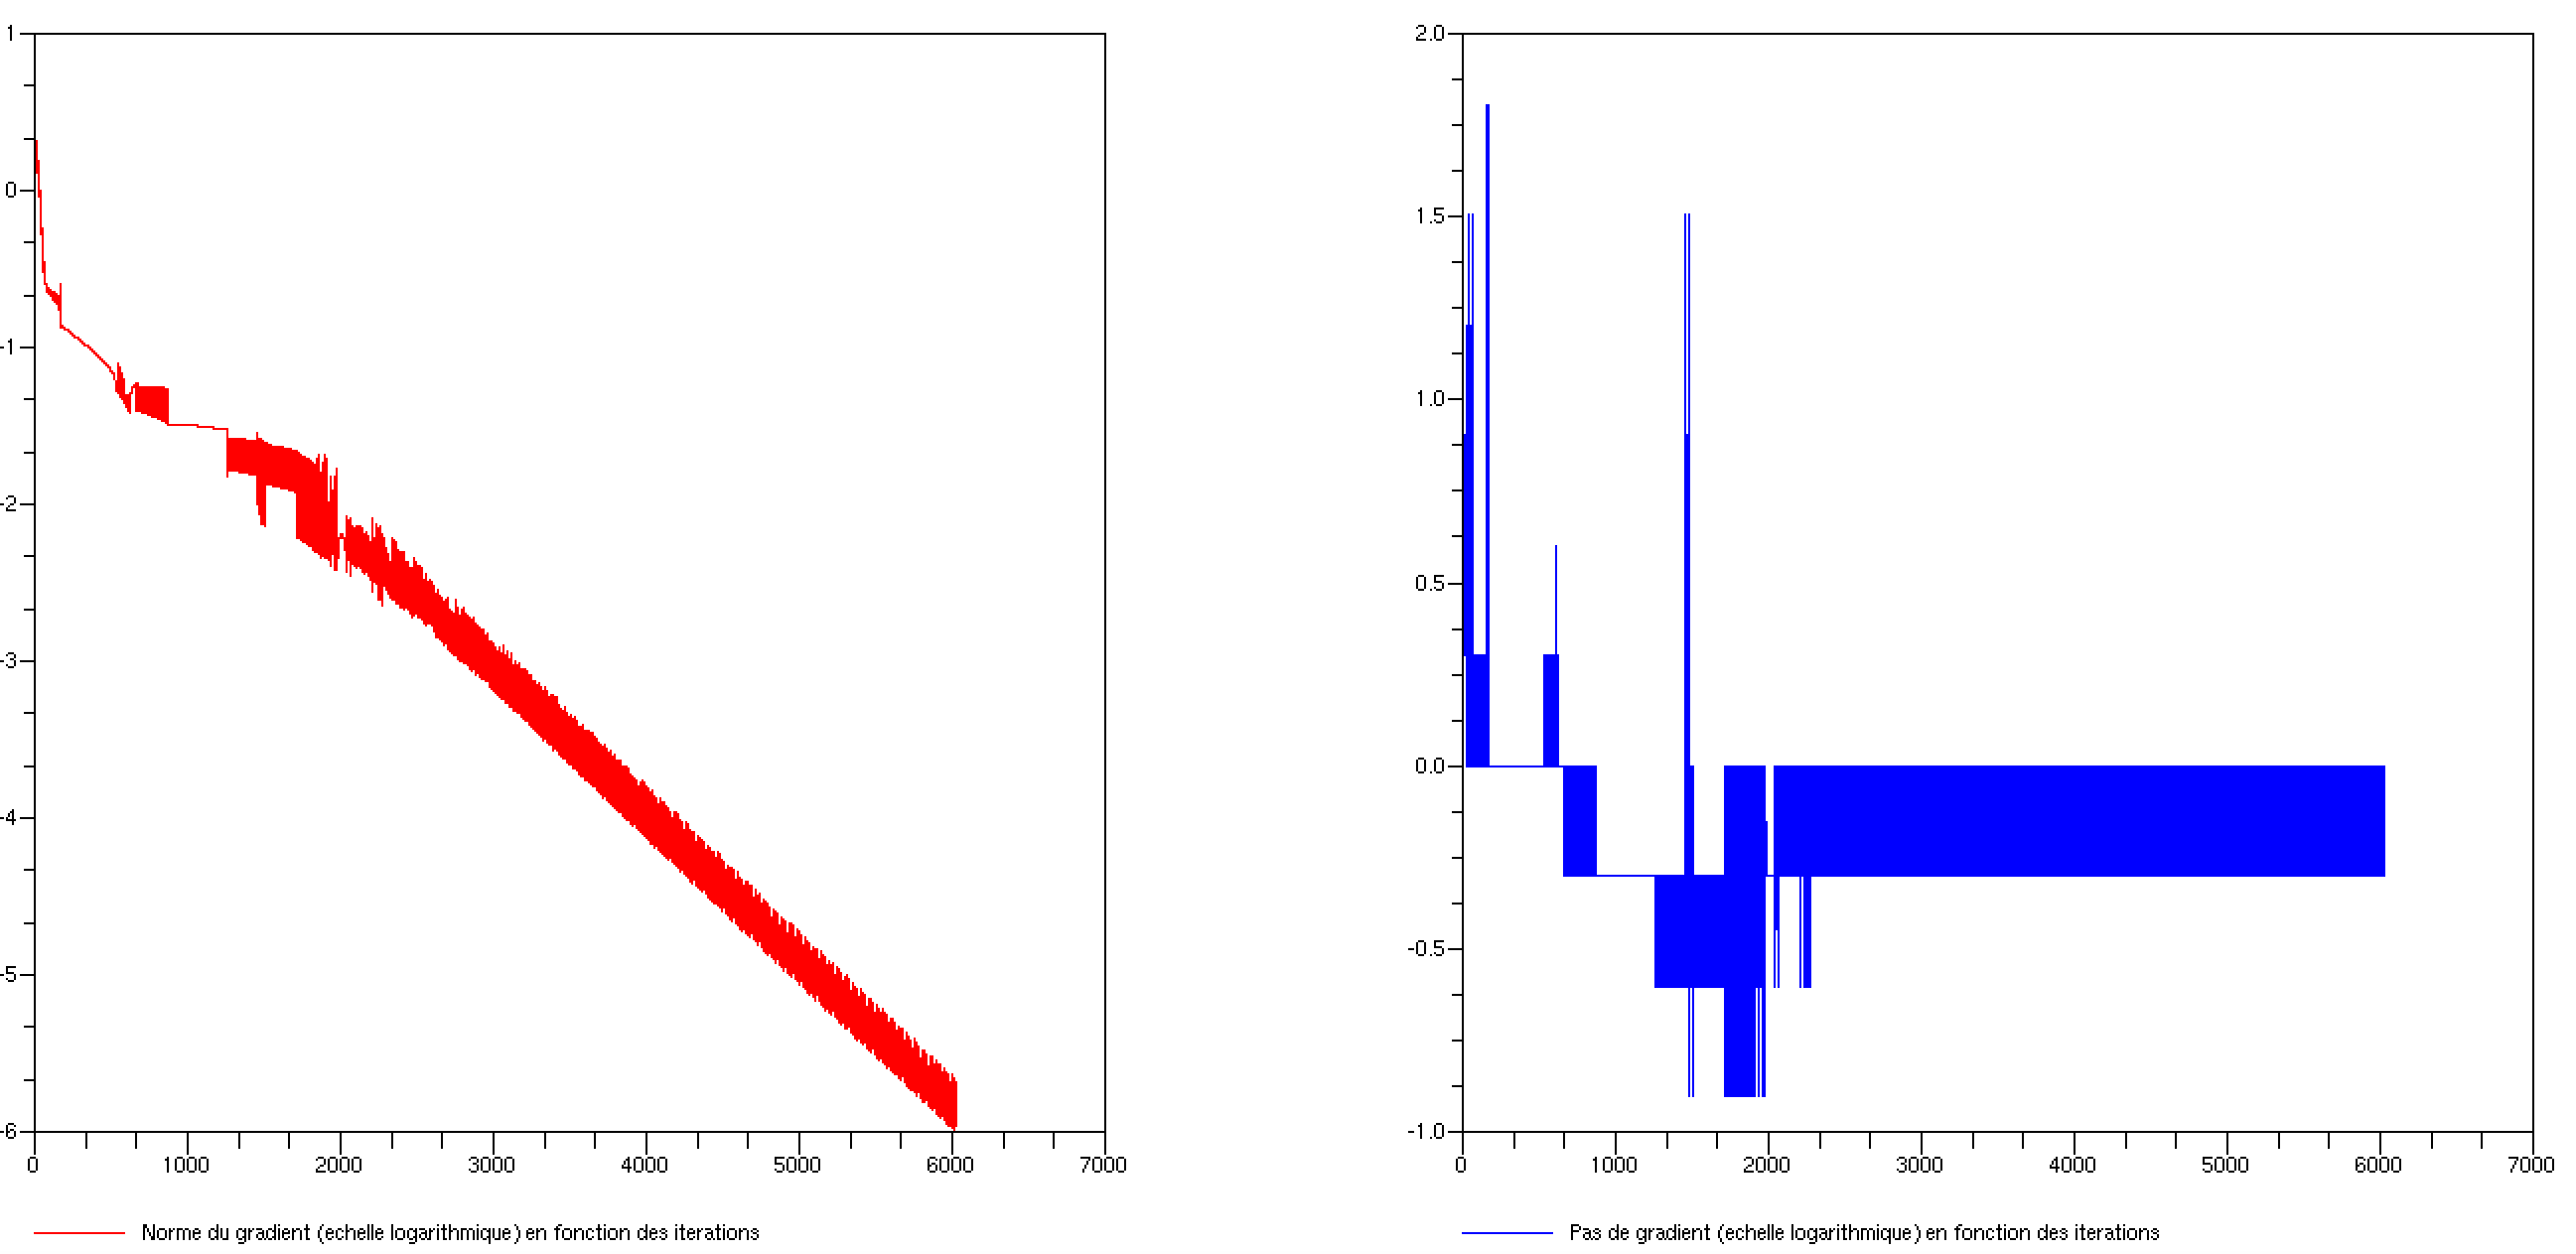
\includegraphics[width=40em,height=15em]{d_wolfe_f.png}
  \captionof{figure}{\small La performance du Gradient à pas variable}
\end{center}

Le gradient à pas variable résout le problème dual mais la vitesse est lente.

\subsection{Polak - Ribière}

\begin{center}
  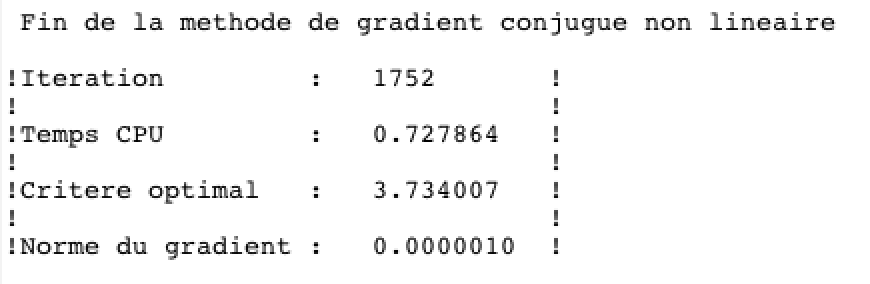
\includegraphics[width=20em,valign=t]{d_conj.png}
  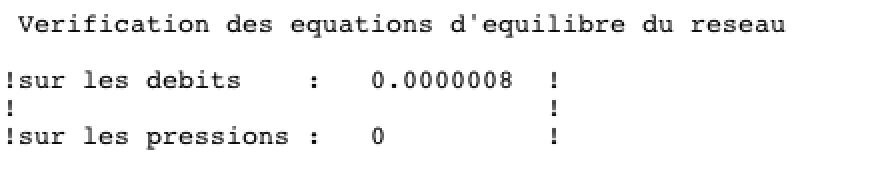
\includegraphics[width=20em,valign=t]{d_conj_v.png}
  \captionof{figure}{\small La performance du Gradient conjugé}

  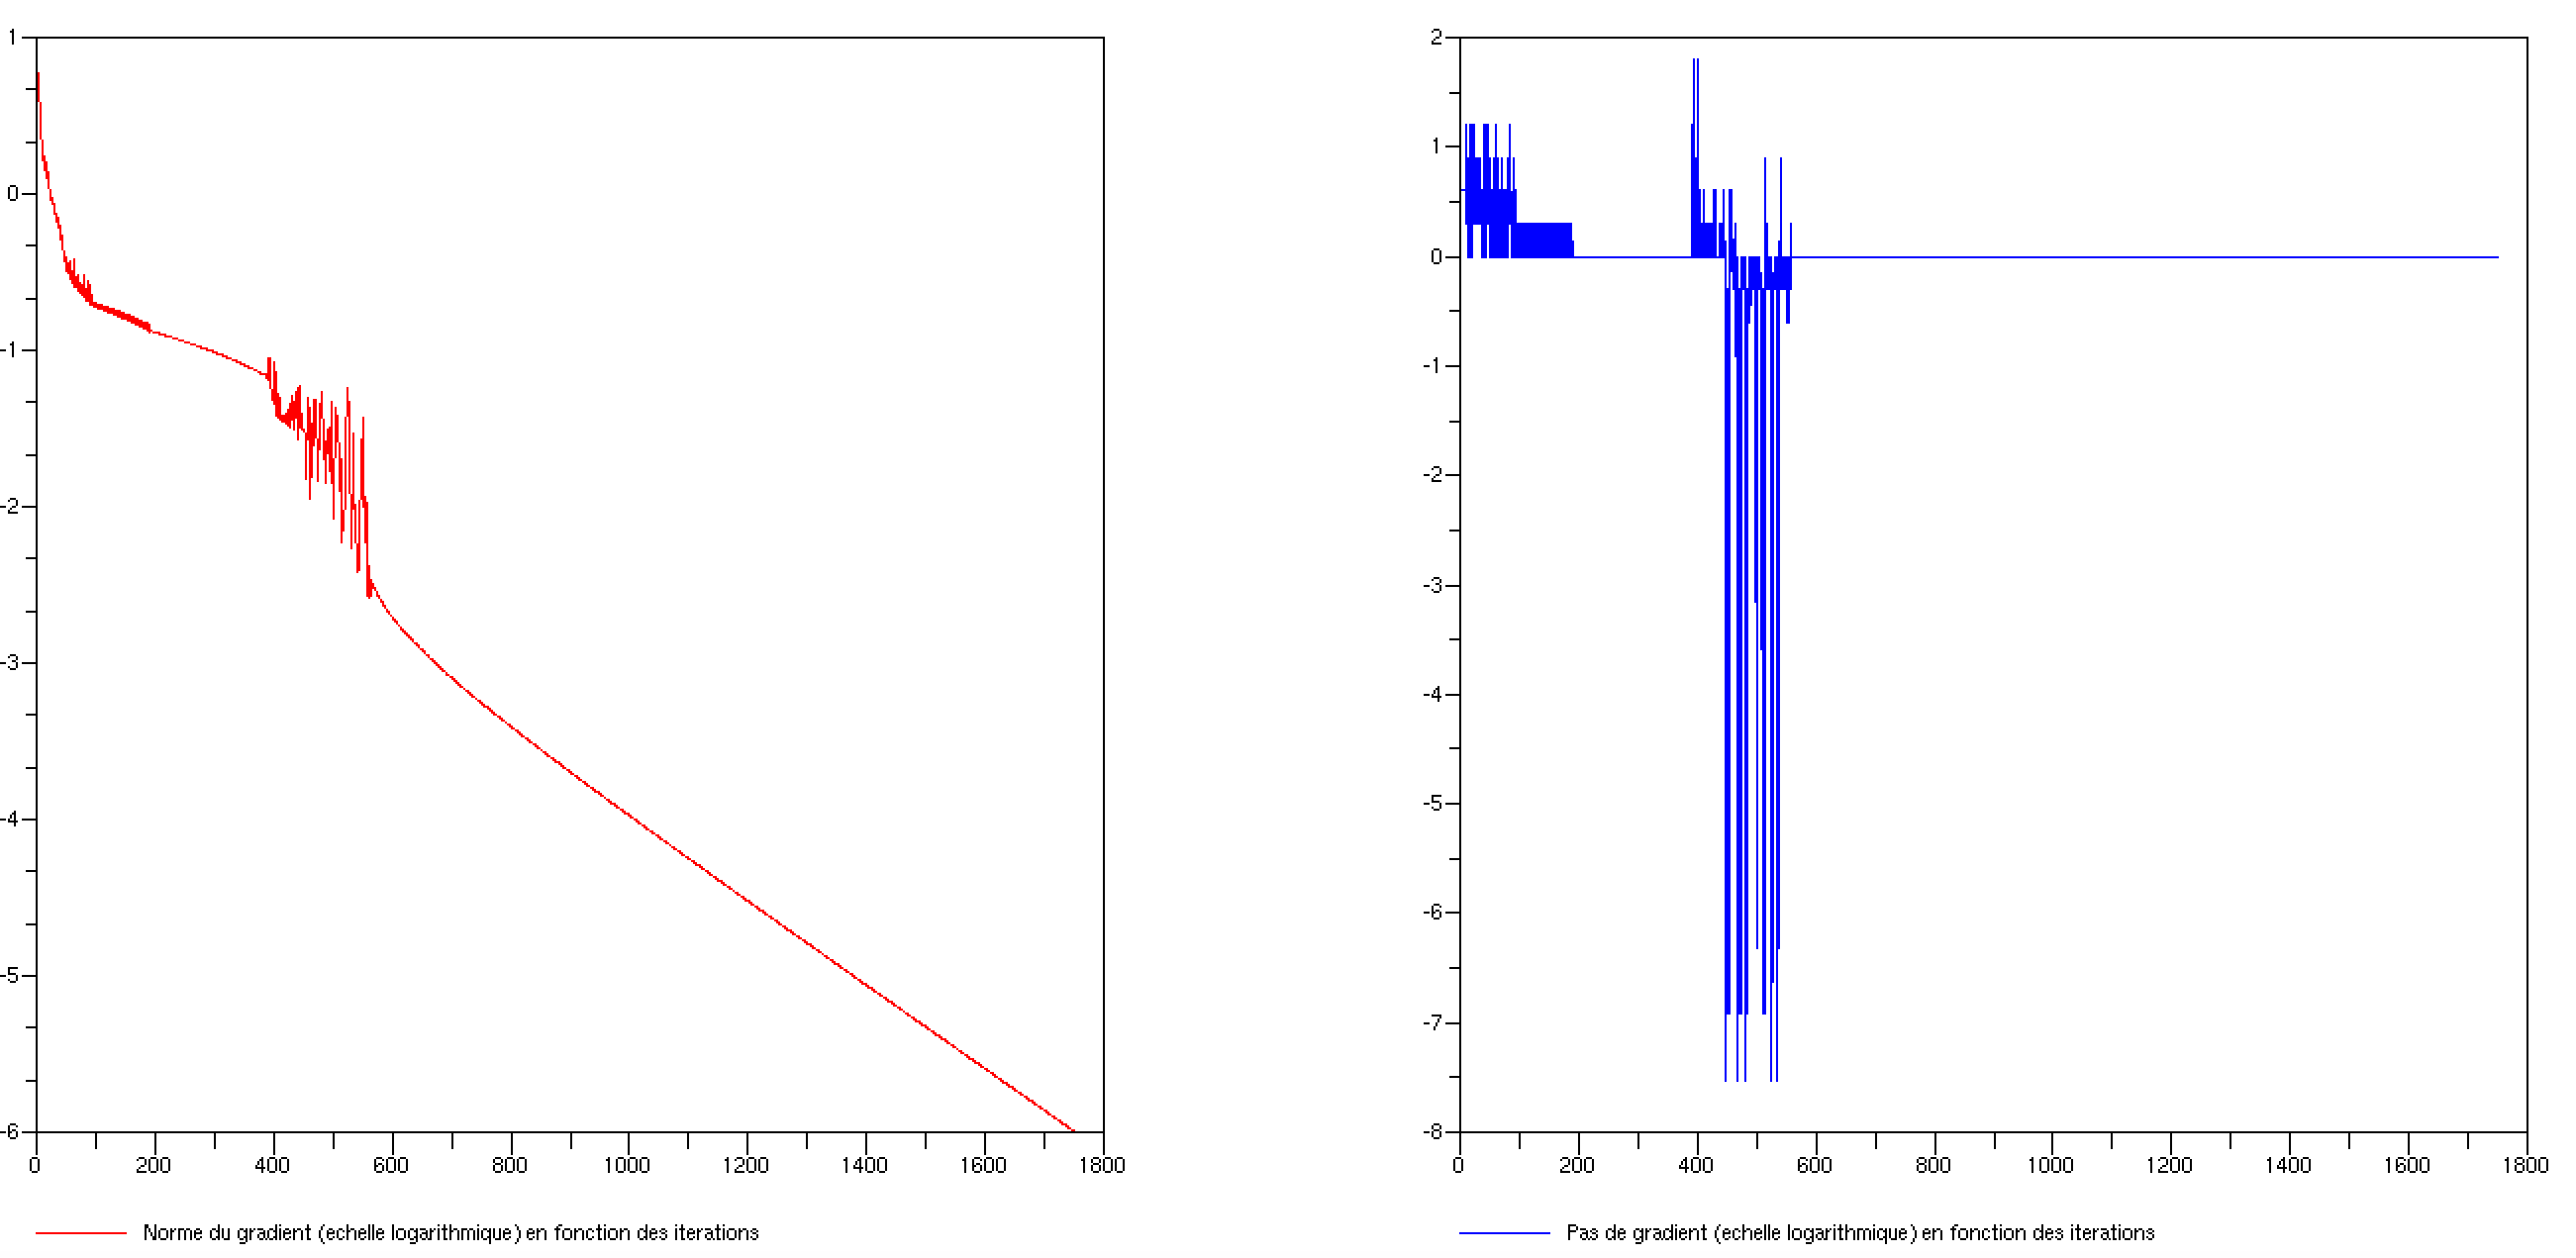
\includegraphics[width=40em,height=15em]{d_conj_f.png}
  \captionof{figure}{\small La performance du Gradient conjugé}
\end{center}

\subsection{BFGS}

\begin{center}
  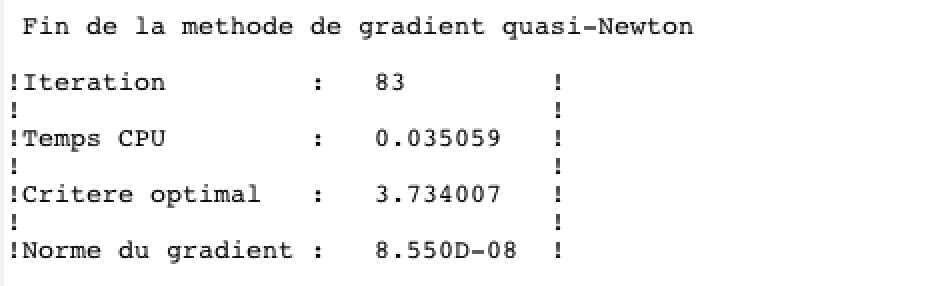
\includegraphics[width=20em,valign=t]{d_quasi.png}
  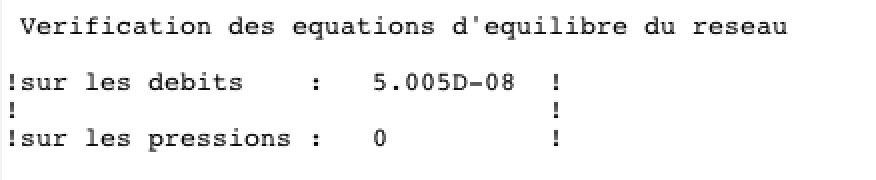
\includegraphics[width=20em,valign=t]{d_quasi_v.png}
  \captionof{figure}{\small La performance du Gradient de Quasi-Newton}

  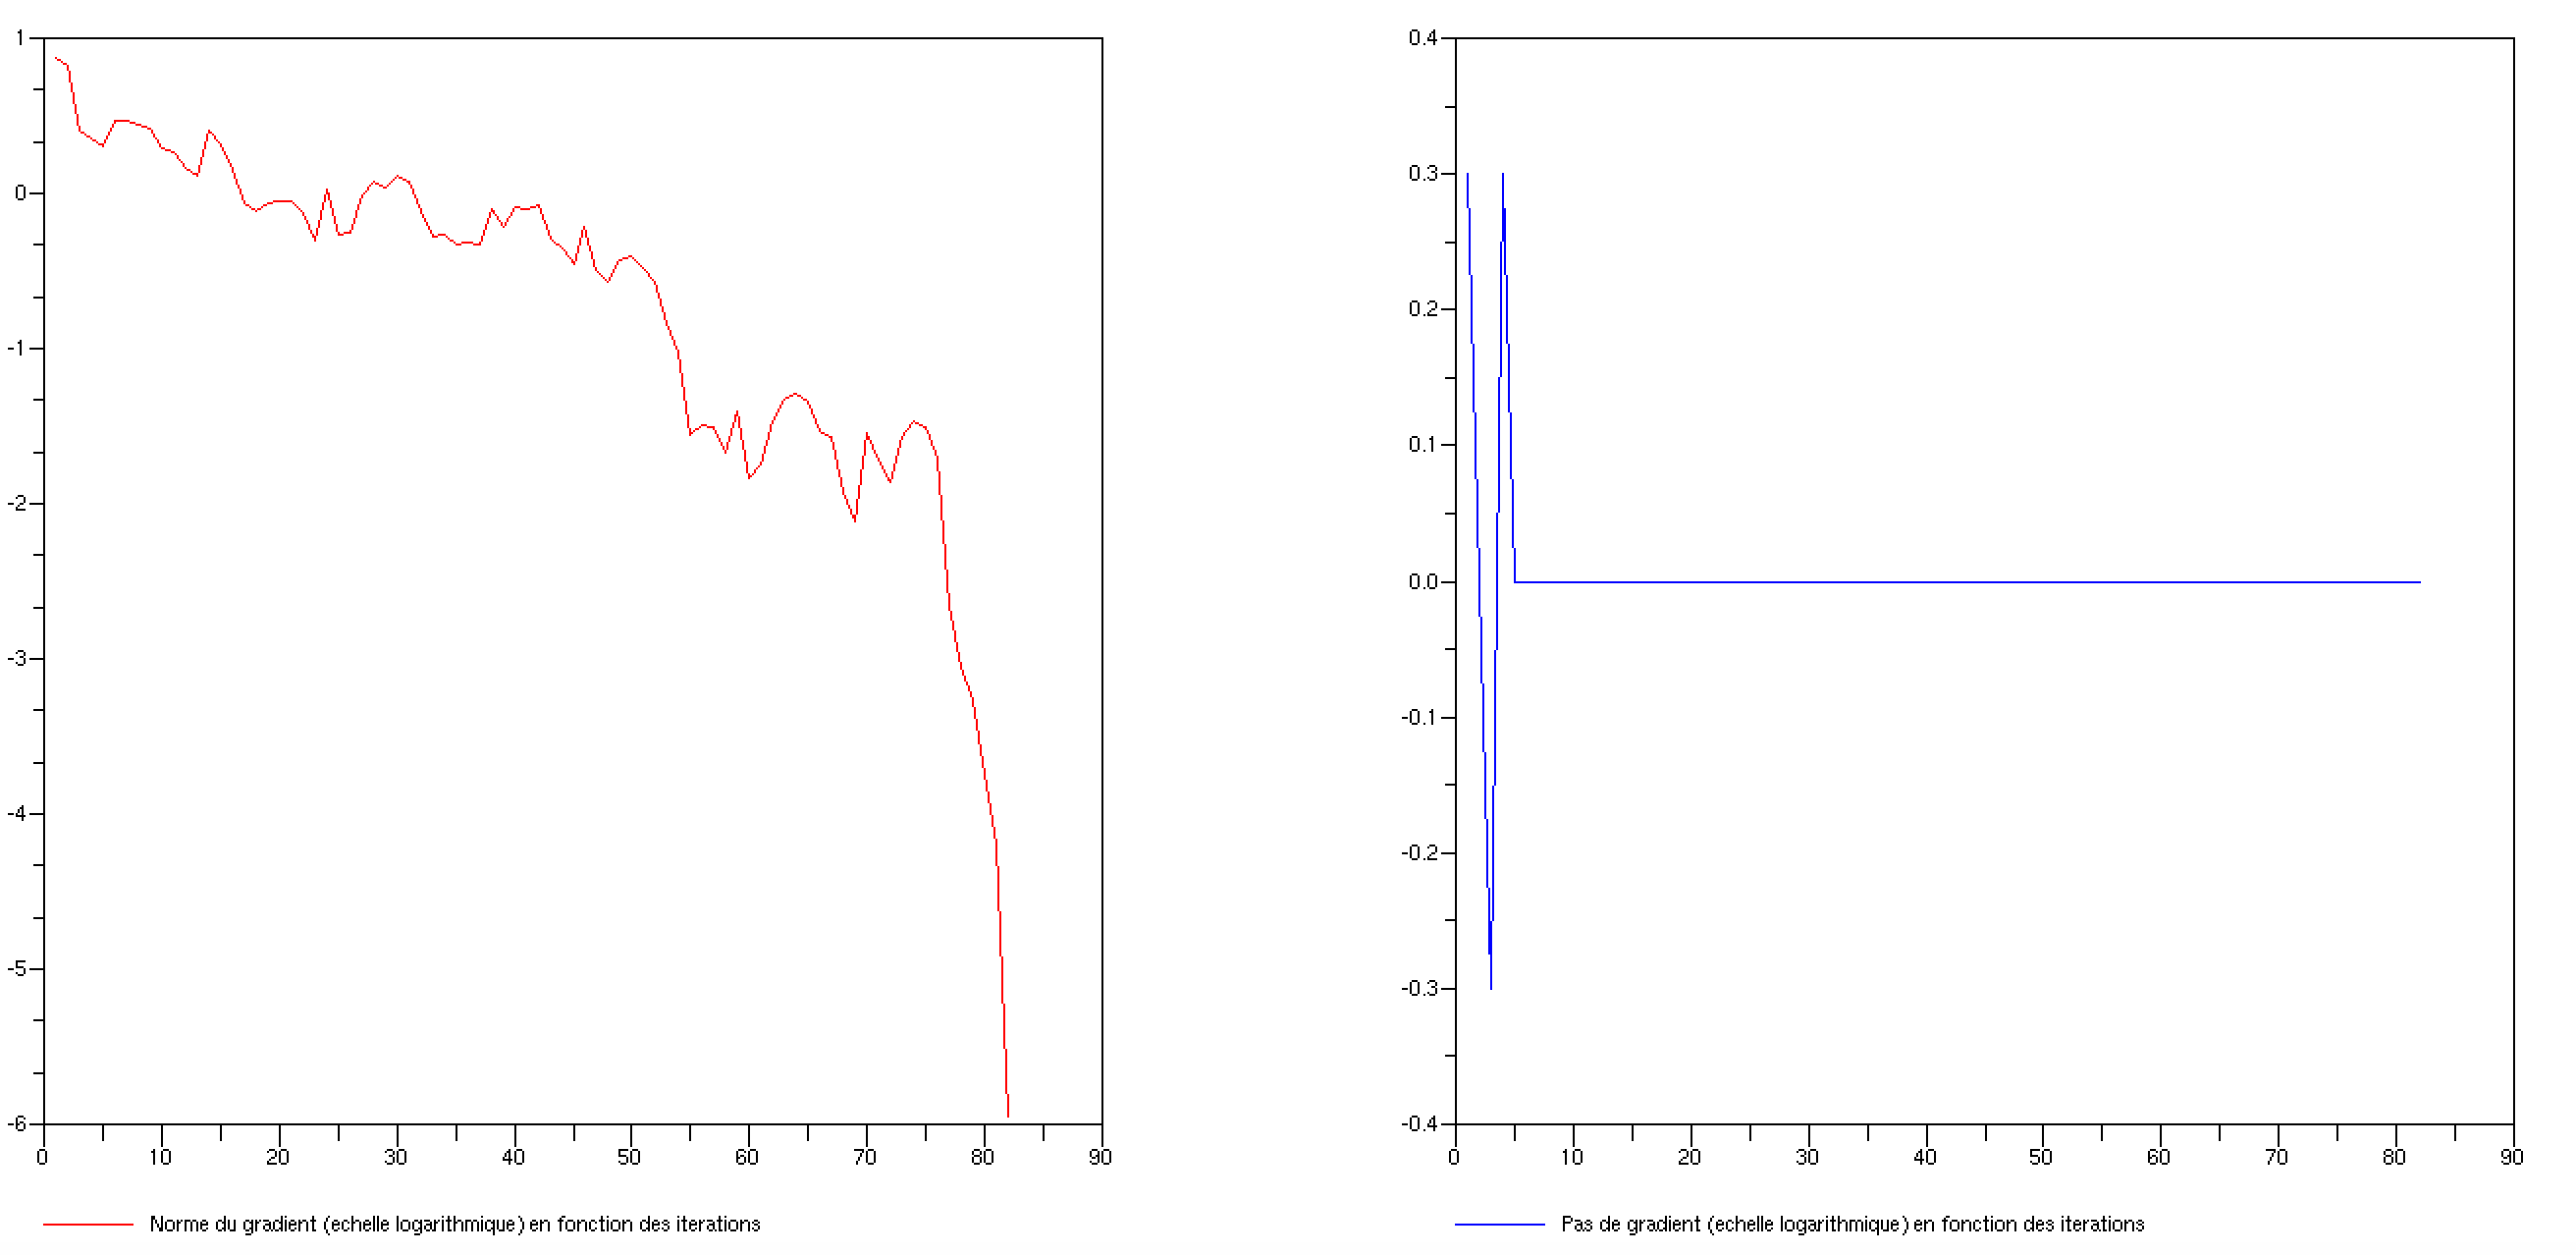
\includegraphics[width=40em,height=15em]{d_quasi_f.png}
  \captionof{figure}{\small La performance du Gradient de Quasi-Newton}
\end{center}

\subsection{Méthode de Newton}

\begin{center}
  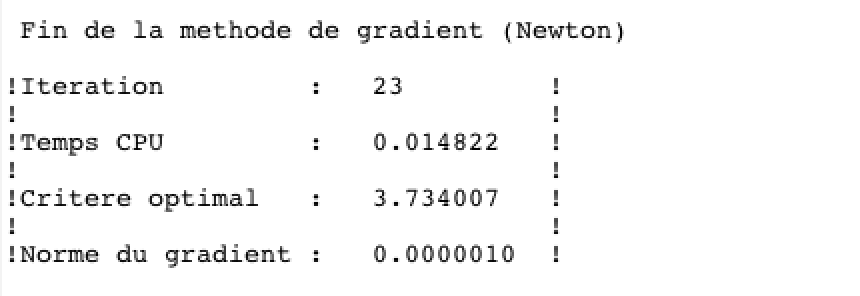
\includegraphics[width=20em,valign=t]{d_newton.png}
  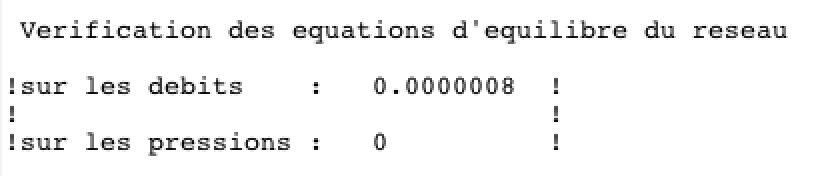
\includegraphics[width=20em,valign=t]{d_newton_v.png}
  \captionof{figure}{\small La performance du Gradient de Newton}

  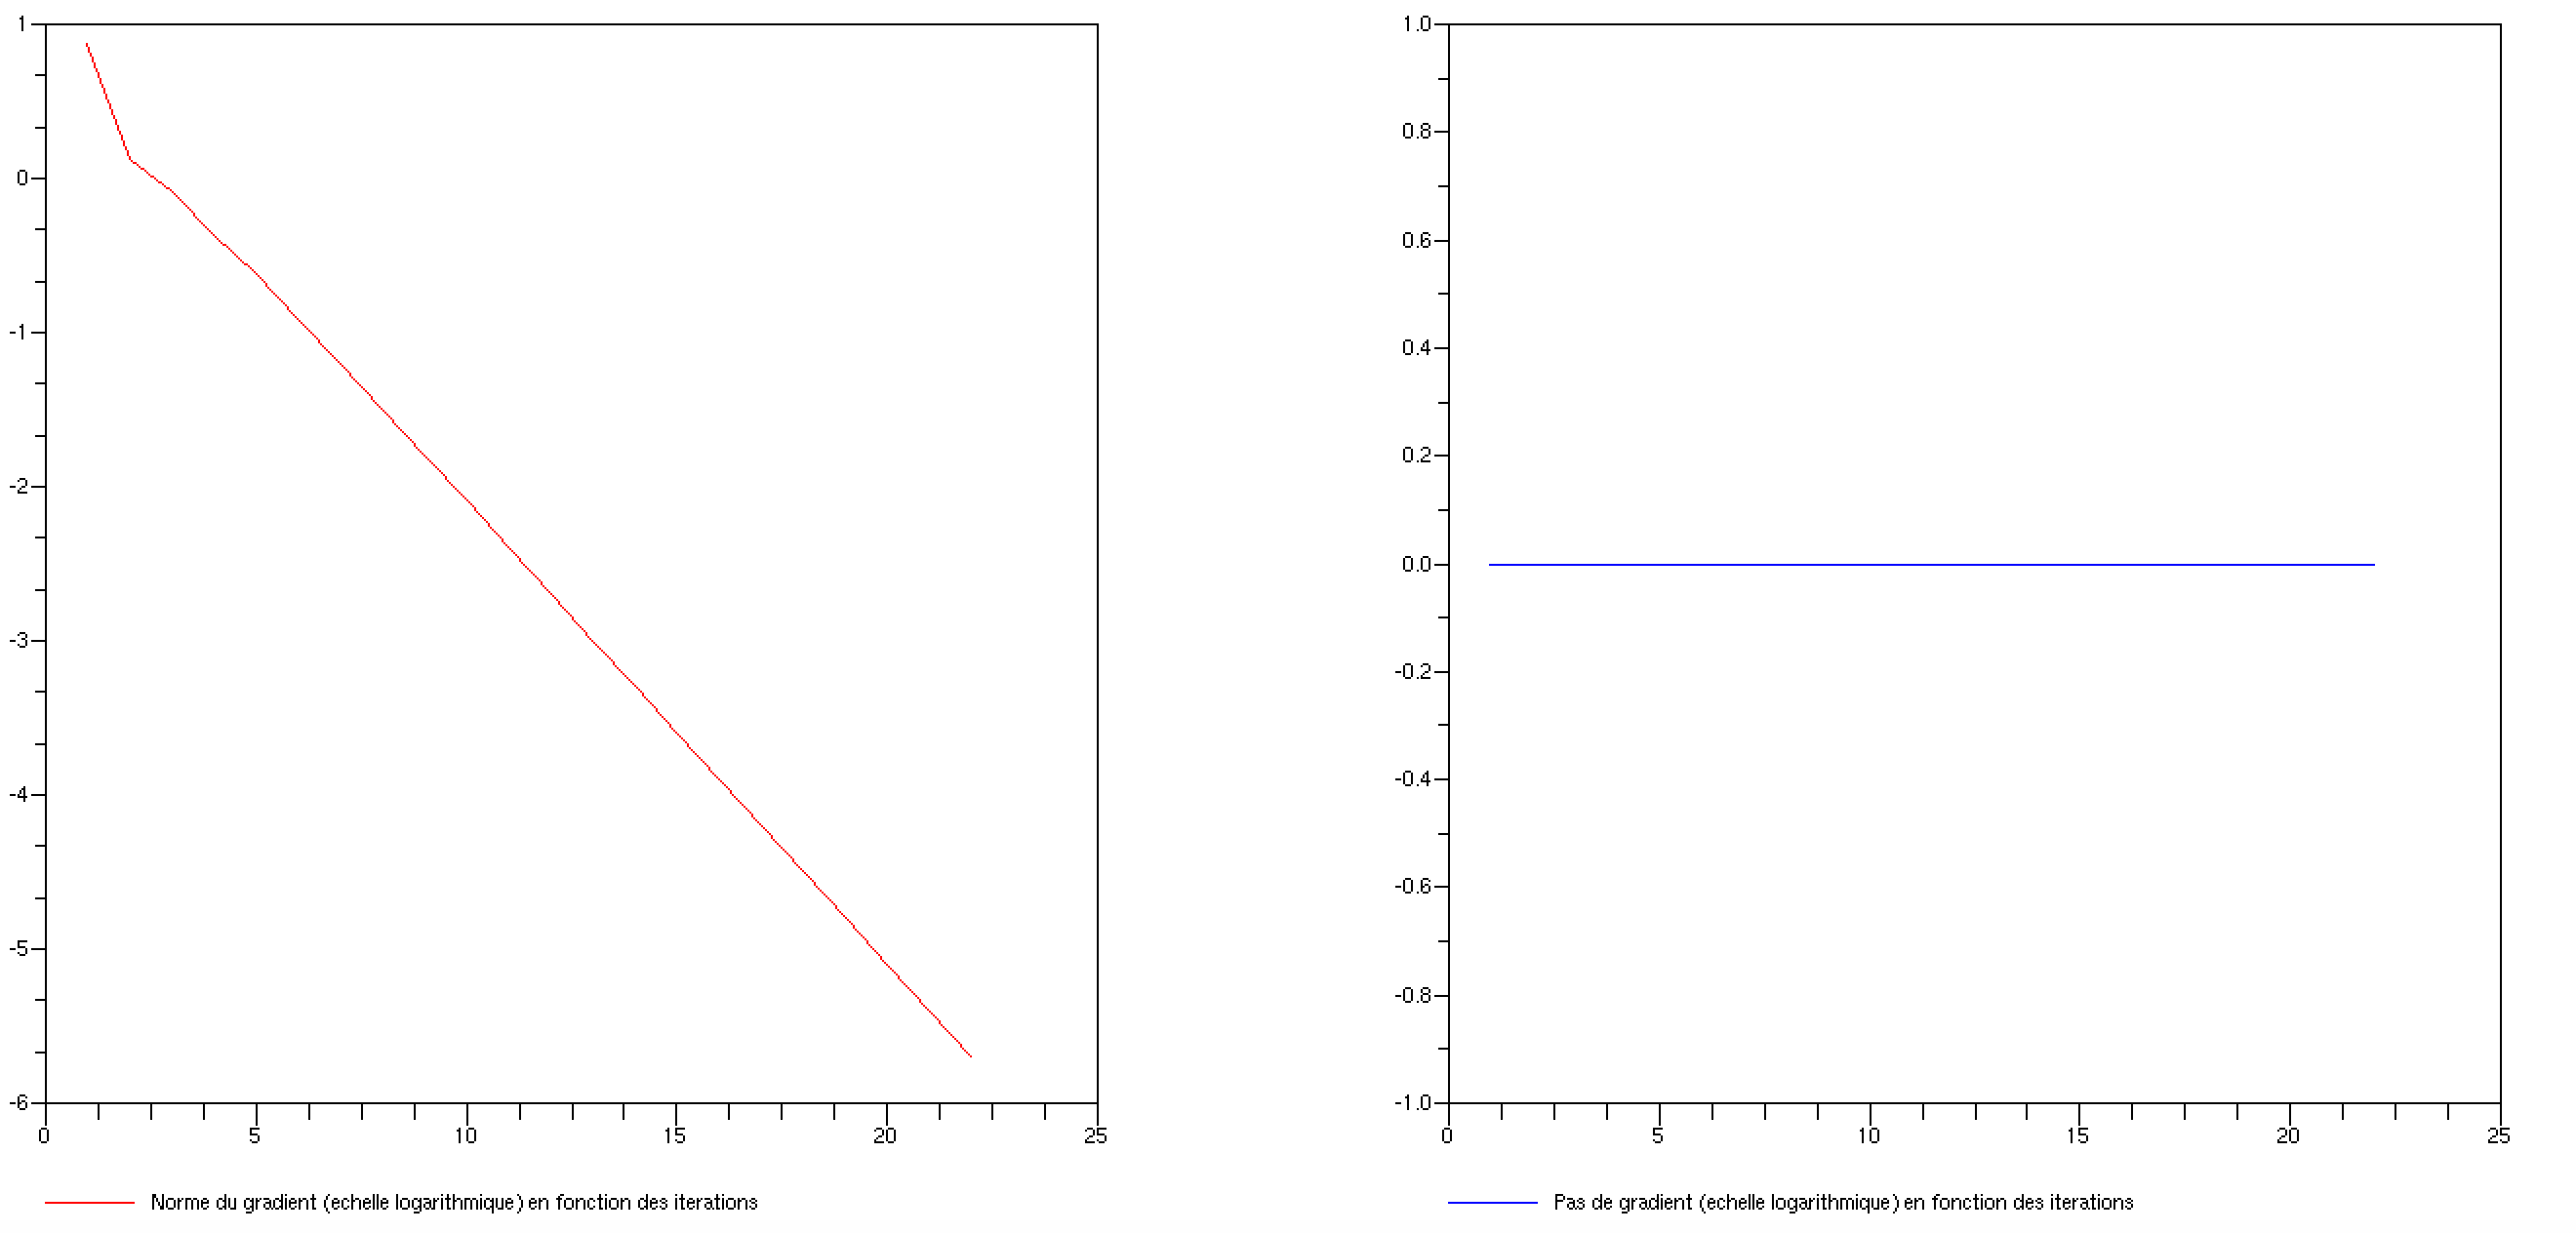
\includegraphics[width=40em,height=15em]{d_newton_f.png}
  \captionof{figure}{\small La performance du Gradient de Newton}
\end{center}

\subsection{Tableau - Comparatif des résultats}

\begin{center}
    \begin{tabular}{| l | c | c | c | c | c |}
    \hline
    Algorithme & Problème & Itération & Temps CPU & Critère optimal & Norme de gradient \\ \hline
      \multirow{2}{*}{La fonction optim de Scilab} & Primal & - & 0.001429 & -3.734007 & 3$\times 10^{-7}$\\ \cline{2-6}
      & Dual & - & 0.007465 & 3.734007 & 5.757$\times 10^{-9}$ \\ \hline
      \multirow{2}{*}{Le gradient à pas fixe} & Primal & 4095 & 0.80611 & -3.734007 & $10^{-6}$ \\ \cline{2-6}
      & Dual & 50000 & 36.236974 & 31.031862 & 0.4505867 \\ \hline
      \multirow{2}{*}{Flechter-Lemaréchal} & Primal & 296 & 0.355025 & -3.734007 & $10^{-6}$\\  \cline{2-6}
      & Dual & 6031 & 2.619408 & 3.734007 & $10^{-6}$ \\ \hline
      \multirow{2}{*}{Polak-Ribière}  & Primal & 177 & 0.248885 & -3.734007 & $7\times 10^{-7}$\\  \cline{2-6}
      & Dual & 1752 & 0.727864 & 3.734007 & $10^{-6}$ \\ \hline
      \multirow{2}{*}{BFGS} & Primal & 22 & 0.019164& -3.734007 & $5\times 10^{-7}$\\ \cline{2-6}
      & Dual & 83 & 0.035059 & 3.734007 & $8.55 \times 10^{-8}$ \\ \hline
      \multirow{2}{*}{L'algorithme de Newton} & Primal & 6 & 0.004687 & -3.734007 & 3.927$\times 10^{-9}$\\ \cline{2-6}
      & Dual & 23 & 0.014822 & 3.734007 & $10^{-6}$ \\ \hline
    \end{tabular}
  \end{center}

  Au travers le tableau, on voit bien que le problème dual est plus difficile à optimiser que le problème primal.

  On en déduit le classement d'algorithmes:

  \begin{center}
    \textbf{Newton > BFGS > Polak-Pibère > Flechter-Lemaréchal > Gradient à pas fixe}
  \end{center}

\end{document}

              